\documentclass[a4paper,12pt]{ctexart}

% ============ 页面与字体 ============
\usepackage[top=2.54cm, bottom=2.54cm, left=3.17cm, right=3.17cm]{geometry}
\usepackage{setspace}
\setlength{\parindent}{2em}
% 正文行距：24磅 ≈ 1.5倍（12pt 字号下）
\linespread{1.5}
\setlength{\parskip}{0pt}

% ============ 数学 ============
\usepackage{amsmath,amssymb,amsfonts}

% ============ 表格与图形 ============
\usepackage{booktabs}
\usepackage{multirow}
\usepackage{graphicx}
\usepackage{float}
\usepackage{caption}
\usepackage{array}
\usepackage{tabularx}
\DeclareCaptionFont{thesiscaption}{\songti\zihao{-4}}
\captionsetup[table]{font=thesiscaption,justification=centering,singlelinecheck=false}
\captionsetup[figure]{font=thesiscaption,justification=centering,singlelinecheck=false}

% 统一插图命令：\myfig[宽度]{图片路径}{图题}{标签}
\newcommand{\myfig}[4][0.85\textwidth]{%
  \begin{figure}[H]
    \centering
    \includegraphics[width=#1]{#2}
    \caption{#3}
    \label{#4}
  \end{figure}
}

% ============ 其他 ============
\usepackage{enumitem}
\usepackage{titlesec}
\usepackage{etoolbox}
\usepackage{indentfirst}
\usepackage{hyperref}
\hypersetup{hidelinks}
\usepackage[superscript]{cite}
\renewcommand\citeleft{[}
\renewcommand\citeright{]}
\renewcommand\citeform[1]{[#1]}
\usepackage{url}
\usepackage[titles]{tocloft}   % 加 titles 选项，避免与 ctex 的章节命令冲突

% 论文题目字体：使用稳定可用的宋体
\setCJKfamilyfont{thesistitle}{STSong}
\newcommand{\thesistitlefont}{\CJKfamily{thesistitle}\fontsize{16pt}{24pt}\selectfont}

% ============ 章节编号 ============
\renewcommand{\thesection}{\chinese{section}}
\renewcommand{\thesubsection}{\arabic{section}.\arabic{subsection}}
\renewcommand{\thesubsubsection}{\arabic{section}.\arabic{subsection}.\arabic{subsubsection}}

% ============ 章节标题格式 ============
\titleformat{\section}[block]
  {\centering\fontsize{15pt}{22pt}\bfseries\heiti}
  {第\thesection 章}{1em}{}
\titlespacing*{\section}{0pt}{18pt}{18pt}

\titleformat{\subsection}
  {\fontsize{14pt}{20pt}\bfseries\heiti}
  {\thesubsection}{1em}{}

\titleformat{\subsubsection}
  {\fontsize{12pt}{18pt}\bfseries\heiti}
  {\thesubsubsection}{1em}{}

% ============ 目录设置 ============
\renewcommand{\contentsname}{目\quad 录}
\renewcommand{\cfttoctitlefont}{\hfil\fontsize{18pt}{24pt}\bfseries\heiti\selectfont}
\renewcommand{\cftaftertoctitle}{\hfil}
\setlength{\cftbeforetoctitleskip}{0pt}
\setlength{\cftaftertoctitleskip}{20pt}

\renewcommand{\cftsecfont}{\normalsize\heiti}
\renewcommand{\cftsecpagefont}{\normalsize\mdseries}
\renewcommand{\cftsecpresnum}{第}
\renewcommand{\cftsecaftersnum}{章}
\renewcommand{\cftsecaftersnumb}{\quad}
\setlength{\cftsecnumwidth}{2.5em}
\renewcommand{\cftsecleader}{\normalfont\cftdotfill{\cftdotsep}}
\setlength{\cftbeforesecskip}{6pt}

\renewcommand{\cftsubsecfont}{\small}
\renewcommand{\cftsubsecpagefont}{\small}
\setlength{\cftsubsecindent}{3em}
\setlength{\cftsubsecnumwidth}{2.2em}
\renewcommand{\cftsubsecleader}{\normalfont\cftdotfill{\cftdotsep}}
\setlength{\cftbeforesubsecskip}{3pt}

\renewcommand{\cftsubsubsecfont}{\small}
\renewcommand{\cftsubsubsecpagefont}{\small}
\setlength{\cftsubsubsecindent}{4em}
\setlength{\cftsubsubsecnumwidth}{2.2em}
\renewcommand{\cftsubsubsecleader}{\normalfont\cftdotfill{\cftdotsep}}
\setlength{\cftbeforesubsubsecskip}{2pt}

\renewcommand{\cftdotsep}{1.5}
\setcounter{tocdepth}{3}
\setcounter{secnumdepth}{3}

% 表格内容单倍行距
\AtBeginEnvironment{table}{\singlespacing}
% 全局保证图片居中
\AtBeginEnvironment{figure}{\centering}

% ============ 页码 ============
\usepackage{fancyhdr}
\pagestyle{fancy}
\fancyhf{}
\fancyfoot[C]{\thepage}
\renewcommand{\headrulewidth}{0pt}

\begin{document}
\zihao{-4}\songti
\pagenumbering{Roman}



% ==================== 封面页 ====================
\thispagestyle{empty}
\begin{center}

\vspace*{1cm}
{\fontsize{14pt}{20pt}\selectfont 作品编号：TJJM20260000000}

\vspace{1.5cm}
{\fontsize{26pt}{36pt}\selectfont\bfseries 2026\,年（第十二届）全国大学生统计建模大赛}

\vspace{2cm}
{\fontsize{22pt}{30pt}\selectfont 参\quad 赛\quad 作\quad 品}

\vspace{3cm}
\renewcommand{\arraystretch}{1.8}
\begin{tabular}{rl}
{\heiti\fontsize{16pt}{24pt}\selectfont 参赛学校：} & {\fangsong\fontsize{16pt}{24pt}\selectfont 兰州大学} \\
{\heiti\fontsize{16pt}{24pt}\selectfont 论文题目：} & {\fangsong\fontsize{16pt}{24pt}\selectfont 半导体存储价格因何而动？供需结构失衡下半导体存储价格的} \\
 & {\fangsong\fontsize{16pt}{24pt}\selectfont 影响因素分析与混合预测} \\
{\heiti\fontsize{16pt}{24pt}\selectfont 参赛队员：} & {\fangsong\fontsize{16pt}{24pt}\selectfont 葛旭东\quad 李悦昊\quad 黎子豪} \\
{\heiti\fontsize{16pt}{24pt}\selectfont 指导老师：} & {\fangsong\fontsize{16pt}{24pt}\selectfont 吴义东\quad} \\
\end{tabular}
\end{center}
\newpage

% ==================== 摘要 ====================
\begin{center}
{\thesistitlefont 半导体存储价格因何而动$?$}\\[6pt]
{\fontsize{12pt}{20pt}\selectfont ——供需结构失衡下存储价格短期波动的多方法因子分析与预测框架建构}
\end{center}

\vspace{12pt}

\noindent{\heiti\zihao{4}摘要}\quad
\\
\hspace*{2em}当前国际竞争格局严峻，我国半导体产业面临着前所未有的挑战。如何突破“卡脖子技术”成为各界专家讨论的焦点。存储芯片占据全球半导体市场25\%至35\%份额，其价格波动对产业链上下游与国家产业基金配置均具有深远影响。在AI算力需求爆炸与中美科技博弈深化的背景下，如何识别价格核心驱动并构建科学预测模型已成为战略议题。然而，传统单变量计量模型在结构断裂面前束手无策，模糊神经网络又受限于专家输入主观性与因果溯源不明，亟需兼顾因子识别、动态结构与价格预测三项能力的系统框架。本研究以2024年4月至2026年2月的113周周度数据为基础，通过构建存储芯片加权综合价格指数，遴选供给、需求、宏观、政策四维度共9个解释变量，基于灰色关联分析、向量自回归、随机森林和XGBoost设计了一种新型的存储芯片价格混合预测框架。本研究的主要贡献在于成功将混频数据输入预测模型中，并取得了良好的预测效果，同时拓展了存储芯片价格的预测方法，为该领域的学术研究提供了新的视角。在现实意义层面，本框架为制造商、下游厂商与政府决策提供可操作的分析工具与实证依据。
\\

\vspace{6pt}
\noindent{\heiti\zihao{-4}关键词：}存储芯片价格；灰色关联分析；向量自回归；随机森林；AI算力投资

\newpage
% ==================== 目录 ====================
\begin{center}
{\heiti\zihao{4}目录}
\end{center}
\vspace{6pt}
\begingroup
\singlespacing
\makeatletter
\@starttoc{toc}
\makeatother
\endgroup
\newpage

% ==================== 表格与插图清单 ====================
\phantomsection
\addcontentsline{toc}{section}{表格与插图清单}
\begin{center}
{\heiti\zihao{-3} 表格与插图清单}
\end{center}
\vspace{6pt}

\noindent 表\,1\quad 变量定义与来源 \\
表\,2\quad 变量描述统计量 \\
表\,3\quad GRA关联度排序（$\rho = 0.5$）\\
表\,4\quad ADF检验结果汇总 \\
表\,5\quad $Y$的预测误差方差分解（\%）\\
表\,6\quad 模型测试集预测误差对比 \\[12pt]
图\,1\quad GRA滞后关联度曲线 \\
图\,2\quad 脉冲响应函数（IRF）结果\\
图\,3\quad 预测误差方差分解（FEVD）\\
图\,4\quad 特征重要性对比 \\
图\,5\quad 训练集拟合表现

\newpage

% ==================== 正文 ====================
\pagenumbering{arabic}
\setcounter{page}{1}

\section{引言}

\subsection{研究背景与动机}
存储芯片是现代信息技术体系的基础性元器件，涵盖DRAM（动态随机存取存储芯片）、NAND Flash（闪存）、SSD（固态硬盘）等主要品类，广泛应用于智能手机、个人电脑、数据中心、汽车电子、人工智能服务器等几乎所有数字化终端。根据世界半导体贸易统计组织的数据，存储芯片长期占据全球半导体市场总营收的25\%至35\%，是半导体产业中规模最大、波动最剧烈的单一细分品类\cite{kang2010}。

已有研究指出，存储芯片市场具有显著的强周期特征。以DRAM为例，其价格在过去十年中经历了多次幅度超过50\%的剧烈涨跌，这种高波动性对产业链上下游造成了深远影响。对上游制造商而言，价格下行意味着营收骤降甚至亏损的困境，因而不得不削减资本开支并推迟扩产计划；而一旦价格反转上行，产能不足又导致供给短缺，进一步加剧价格波动，形成恶性循环。对下游终端厂商而言，存储芯片通常占据其物料成本的20\%至40\%，异常波动将直接侵蚀终端产品的利润空间。对政府投资决策而言，中国近年来在存储芯片领域投入了大量产业资金，价格的周期性波动将直接影响相关企业的盈利前景和投资回报周期，进而影响国家产业基金的配置效率与后续投资节奏。

而在当前全球数字经济加速发展的背景下，存储芯片的战略地位进一步凸显。一方面，以ChatGPT为代表的大语言模型（LLM）训练与推理对高带宽存储芯片及大容量SSD的需求呈指数级增长，AI算力基础设施的建设正在重塑存储市场的需求结构。另一方面，我国作为全球最大的存储芯片消费市场，进口依赖度长期处于高位。2019 年以来，美国政府频频出手制裁中国高新技术企业，破坏了基于全球产业大循环的中国半导体产业链，以期从战略上削弱中国制造在高科技领域中的竞争力\cite{wuxiaobo2021}。在中美科技博弈持续深化，美国对华半导体出口管制不断升级的地缘政治格局下，存储芯片的供给安全与价格稳定已上升为关乎国家数字经济安全的战略性议题\cite{luo2023}。在当前背景下，如何准确地分辨出其影响因子，并以此为基础构建科学的价格预测模型，已成为亟需解决的问题。

\subsection{文献综述}
\subsubsection{存储芯片价格影响因素与历史定价法则}

半导体产业是基础性、先导性产业，涉及国家信息安全。有学者认为美国90年代的崛起跟半导体产业的兴盛分不开，经济增长受到半导体设备制造业的进步等的推动。冯昭奎对日本半导体行业的崛起进行了分析，认为芯片技术有着浓重的政治、战略色彩\cite{feng2019}。同时鉴于其产业重要性，探究半导体产业周期及存储芯片价格的驱动因子，始终是学术界的重要议题。

早期研究逐渐归纳出两大经典概念用以推测其价格和利润空间。半导体价格在大规模生产初期相对较高，但随着技术进步而逐渐降低，当产值达到峰值，价格也达到最有利可图的区间\cite{lepselter1985}。同时无论技术取得多大突破，新款半导体最终的稳定价格也只会是老款的两倍\cite{tarui1991}。基于此，业内逐渐建立起依靠经验法则进行定价的主流方法。然而，随着全球化分工深化与市场日趋复杂，单纯依赖技术代际与经验法则的定价机制逐渐失效。

为克服主观经验定价的局限性并提升预测的科学性，学术界与产业界开始转向基于数据的定量预测模型，并将驱动因子的观测范围从单一的技术代际向宏微观经济指标拓展。例如有学者曾揭示了库存水位和晶圆厂产能对产业周期的结构性影响，证实产能过剩与库存周转是触发价格反转的关键先行指标\cite{liu2005}。全球地缘政治风险与全球经济政策不确定性对宏观经济情况和微观行业运行均有所影响\cite{pulin2020}。除此之外，资本支出作为沉没成本与固定投入，其周期性扩张与收缩不仅决定了头部制造厂商的运营效率，更构成了主导存储芯片中长期定价周期的非线性供给约束\cite{qiao2021}。全球广义货币流动性、美元融资约束及宏观汇率波动，同样可以对包括半导体在内的大宗高科技元器件定价产生直接而深远的跨市场溢出效应与非对称冲击\cite{park2025}。现有最新研究将厂商的库存周转天数与宏观指标等变量结合纳入模型，显示出外生变量对DRAM短期价格拟合的显著解释力\cite{hsu2025}。

经此不难发现，当前的存储价格已非仅可通过个体经验进行把握，而是演变为一个高度交织了产业库存、宏观经济景气度以及国际政治经济环境冲击的多因子复杂系统。如何在确保信息不丢失的前提下提取有效信息并剔除市场噪音，是建立高精度模型的核心挑战。

\subsubsection{存储芯片价格预测模型归纳}
在实证方法论上，存储芯片价格预测模型的设计同样经历了一条不断演化的脉络。早期研究多采用单变量ARIMA模型或指数平滑法，其对短期线性趋势拟合良好，但由于半导体产品的定价机制存在高度的非线性与状态依赖性，单变量模型表现乏力\cite{liu2005}。有学者通过引入向量自回归及贝叶斯模型以捕捉多变量领先指标的联动效应，以补充其缺陷\cite{liu2018}。同时，为刻画价格收益率波动的杠杆效应与波动聚集特征，混频数据抽样模型被广泛引入，以评估宏观冲击对半导体市场波动率的非对称影响\cite{snarska2025}。实践证明，在相对稳定且线性发展的市场环境下，这些方法确实展现出较高的准确性与较强的经济学可解释性。然而传统计量模型仍强烈依赖时间序列的历史平稳性假设，在面对由地缘政策或技术突发引发的结构断裂时，往往束手无策。


随着数理统计的深入和机器学习的广泛应用，越来越多的人将现代预测方法应用于价格预测中，如神经网络预测、决策树预测、支持向量机预测、逻辑回顾预测、深度学习预测等。而近十多年来，为了应对价格的非线性波动特征，融合模糊逻辑与协同预测思想的混合模型逐渐成为研究焦点。台湾学者陈东旭率先将混合模糊神经网络应用于存储芯片价格预测\cite{chen2013}，后续研究结合模糊线性回归与反向传播神经网络进行去模糊化处理，结果证实该方法的预测精度优于传统ARIMA模型\cite{chen2014}。针对多专家意见的有效整合问题，其后来的研究提出了分层偏共识模糊协同方法\cite{chen2016}，并在此基础上通过引入区间值模糊数构建了模糊协同预测模型，使盈利预测的准确性得到了进一步提升\cite{chen2021}。

但同时，此类模型存在显著的理论与实践瓶颈。首先，模糊逻辑模型极度依赖专家的主观输入来定义模糊集，导致方法带有强烈的个人意愿且难以规模化。确定区间值模糊数需要极深的行业资历，这在专家意见匮乏或不可靠的极端市场动荡期显得较为不实用。其次，人工神经网络模型在高度波动、充满噪音的半导体市场中，不仅需要规模庞大且具有良好代表性的训练集，而且极易过拟合。在半导体产业中，由于制程迭代加快，旧技术的历史价格轨迹很难直接映射到新技术上。神经网络模型的黑盒特性更是难以解释突发的市场破坏或技术换代冲击，对各项输入特征的影响因子分析不明，极大地限制了其在宏观产业决策与具有明确因果溯源要求的政策预算中的应用价值。


\subsection{研究内容及创新点}

针对上述不足，本研究提出了一种三阶段混合分析与预测框架。第一阶段以灰色关联分析（GRA）作为因素初筛与滞后识别工具，在不假设线性或特定分布的条件下对候选变量进行排序与时滞标定。第二阶段引入向量自回归（VAR）模型，通过脉冲响应函数（IRF）与预测误差方差分解（FEVD）定量刻画变量间的动态因果结构。第三阶段以XGBoost与随机森林两种非线性集成学习模型完成短期价格预测，并通过反RMSE加权将VAR、随机森林与XGBoost的预测输出进行集成\cite{wang2023}。

在创新层面，本文的创新点主要体现在两个方面。其一，在变量设计层面，本文构建了覆盖供给、需求、宏观与政策四维度的候选解释变量集合，并通过GRA关联度排名、FEVD贡献分解、随机森林Gini重要性和XGBoost增益重要性四种独立度量进行因素重要性的交叉验证，克服了以往研究中单一方法因子排序缺乏稳健性保障的缺陷。其二，在方法论层面，本文将GRA的变量筛选与特征滞后期$\tau_i^*$嵌入机器学习模型的特征工程，使灰色系统理论的输出直接指导后续非线性模型的输入构造，实现了灰色系统理论与机器学习之间的衔接，避免了机器学习模型在高维小样本条件下常见的过拟合问题。

% ==================== 第二章 ====================
\section{数据来源与变量设计}

\subsection{存储芯片综合价格指标}

为构建有效的预测模型，本文自DRAMeXchange、TrendForce及Bloomberg存储芯片板块终端采集NAND Flash、DRAM与SSD三类主要存储芯片的现货与合约报价。考虑到2024年以来全球存储芯片市场先后经历下行探底、触底企稳至有序上行的完整周期，并兼顾云厂商AI资本支出对需求端的结构性重塑，样本期确定为2024年1月1日至2026年2月28日，以每周周五为基准对齐，共得到113个周度观测点。

被解释变量$Y_t$为NAND Flash、DRAM与SSD三类存储芯片构造的加权价格指数，权重依据2024至2025年全球存储芯片市场结构设定为$\omega_{\text{NAND}}=11.1\%$、$\omega_{\text{DRAM}}=56.7\%$、$\omega_{\text{SSD}}=32.2\%$，并以样本首期为基期标准化至100：
\begin{equation}
Y_t = 100 \times \frac{\omega_N P_t^N + \omega_D P_t^D + \omega_S P_t^S}{\omega_N P_0^N + \omega_D P_0^D + \omega_S P_0^S}
\end{equation}

其中$P_t^N$、$P_t^D$、$P_t^S$分别为每周NAND、DRAM与SSD的均价。权重结构参考Bank of America与世界半导体贸易统计组织（WSTS）2025至2026年度结构报告中对三类产品的全球销售额占比估算，并于样本期内保持固定，以避免权重内生波动对指数动态的干扰。最终样本中，训练集取2024年1月至2025年12月共约105周，覆盖存储芯片周期由下行探底到有序上行的完整阶段。测试集取2026年1月至2月共8周，用于样本外预测评估。


\subsection{核心解释变量}

基于以往存储芯片周期研究的理论框架，本文从供给侧、需求侧、宏观经济环境与政策四个维度构建候选解释变量集合，初始共纳入6个自变量与5个中介变量。经后文共线性诊断剔除$X_5$与$M_5$后，最终进入模型的变量共9个。各变量的经济含义、数据来源与量纲如表\,1所示。

其中$X_1$为英伟达、微软、亚马逊、谷歌、Meta五大云算力服务商的季度资本支出和，本研究将该指标作为研判AI算力需求强度最被广泛接受的前瞻性信号。$X_2$为三星电子、SK海力士与美光三大制造商的季度运行成本和存货合计，用于度量供给端的边际成本和库存情况。$X_3$取自公开的EPU指数，用以刻画中美科技博弈、关税政策、出口管制等事件对存储芯片贸易条件的冲击。$X_4$采用洲际交易所布伦特原油日度结算价，以反映上游能源成本与晶圆制程电费的传导路径。$X_6$为外生确定性变量，刻画2023年存储芯片行业减产承诺的产能恢复进度，采用指数衰减函数$X_6(t)=5+30e^{-\lambda w}$构造，其中$\lambda = \ln 2/78$，$w$为自2024年1月1日以来的周数。

在中介变量设计上，$M_1$为HBM占DRAM总产能的比重，度量制造商将传统DRAM产能转向高附加值HBM的结构性替代程度。随着AI大模型对高带宽内存的需求急剧攀升，三星、SK海力士和美光均将大量DRAM产线切换至HBM制程，这一结构性产能迁移直接压缩了传统DDR产品的可用产能，成为推升存储芯片价格的重要供给侧因素。$M_2$以美光库存天数的同比变化率取反作为行业供需缺口的代理，当其同比下降时意味着去库存加速，需求超过供给，反之则为过剩。$M_3$为美光合约负债，主要反映已收取但未确认收入的长单预收款，构成价格的前瞻性需求指标。当合约负债显著增加时，表明下游客户提前锁定未来供货，预示后续需求将保持强劲。$M_4$为美国半导体与相关器件制造业生产者价格指数，用于控制行业整体价格中枢的变动。

% ===== 表1 =====
\begin{table}[H]
\centering
\renewcommand{\arraystretch}{1.2}
\footnotesize
\begin{tabular}{cllll}
\toprule
变量代码 & 变量名 & 经济含义 & 数据源 & 量纲 \\
\midrule
$Y$ & 存储芯片综合价格指数 & 被解释变量 & Bloomberg与 TrendForce & 指数 \\
$X_1$ & 云厂商资本支出 & AI需求动能 & 各公司季度财报 & 亿美元 \\
$X_2$ & 制造商成本与库存 & 供给端成本 & 各公司季度财报 & 亿美元 \\
$X_3$ & 经济政策不确定性 & 政策风险 & EPU数据库 & 指数 \\
$X_4$ & 布伦特原油价格 & 能源成本 & U.S.\ EIA & 美元/桶 \\
$X_5$ & 晶圆厂建设倒计时 & 产能扩张预期 & 本文测算 & 无量纲 \\
$X_6$ & 历史减产产能恢复衰减 & 供给收缩效应 & 本文测算 & 无量纲 \\
$M_1$ & HBM产能挤占 & 产能结构替代 & TrendForce与 SEMI & 百分比 \\
$M_2$ & 供需缺口 & 行业平衡 & 美光季度指标 & 百分比 \\
$M_3$ & 合约负债 & 订单前瞻 & 美光季度财报 & 亿美元 \\
$M_4$ & 半导体PPI & 行业价格水准 & FRED数据库 & 指数 \\
\bottomrule
\end{tabular}
\caption{变量定义与来源}
\label{tab:variables}
\end{table}

\subsection{数据预处理}

由于变量原始频率不统一，且季度财报具有发布时滞，本研究采用五类技术将所有变量对齐至以周五为基准的周度网格。日频序列（$Y$、$X_3$、$X_4$）取周内均值以平滑日间噪声，同时保留周度内的信息密度。月频序列（$M_4$）采用线性插值，因半导体生产者价格指数反映的是平滑的潜在价格过程，其月内变动通常呈近似线性特征，线性插值可在不引入虚假高频波动的前提下完成频率转换。季频数据（$X_1$、$X_2$、$M_2$、$M_3$）来源于上市公司季度财务报告，其发布日期通常滞后于报告期末约30至60天。若直接将季报数据对应至报告期内的各周，模型将在训练阶段使用尚未公开的信息，导致前瞻性偏差。为此，本文采用阶梯函数并施加45天发布滞后，即每季度报告期结束后45天内沿用上季数值，确保模型在任何时间点使用的均为当时已公开可得的信息。年频序列（$M_1$）采用三次样条插值，因HBM产能占比反映的是技术转型驱动的缓慢产能迁移过程，其年内变动轨迹具有连续可微的平滑特征，三次样条函数可较好地逼近这一潜在过程。$X_6$为解析函数，直接在周度网格上求值。

\subsection{共线性筛除}
在初始候选变量集合中，为避免多重共线性对VAR方程系数识别与脉冲响应方向的扭曲，本研究以方差膨胀因子（Variance Inflation Factor, VIF）作为诊断指标：
\begin{equation}
\text{VIF}_j = \frac{1}{1-R_j^2}
\end{equation}

其中 $R_j^2$ 为以第 $j$个解释变量对其余解释变量做OLS辅助回归的判定系数。按照计量经济学通行标准，$\mathrm{VIF}_j > 10$ 表示严重共线性，$5 < \mathrm{VIF}_j \le 10$表示中度共线性。经诊断， $X_5$ 与 $M_3$ 的相关系数达$0.91$、$\mathrm{VIF}(X_5)=14.8$。出于保留前瞻信息较强者的原则，以及为了避免影响模型精度，因而剔除 $X_5$，保留 $M_3$。剔除后剩余变量均降至4.2以下，满足VAR建模的弱共线性要求。

\subsection{整体变量描述}
表\,2报告了最终10个变量在全样本期（$N=113$周）的描述统计量。Jarque-Bera检验显示大部分变量显著拒绝正态假设（$p<0.01$），表明针对具有非正态、尖峰特征的序列，采用不依赖分布假设的GRA与机器学习模型具备适配优势。

% ===== 表2 =====
\begin{table}[H]
\centering
\renewcommand{\arraystretch}{1.15}
\footnotesize
\begin{tabular}{lrrrrrr}
\toprule
变量 & 均值 & 标准差 & 最小值 & 最大值 & 偏度 & 峰度 \\
\midrule
$Y$ & 108.43 & 16.72 & 84.56 & 158.21 & 1.28 & 4.17 \\
$X_1$ & 652.30 & 187.44 & 391.20 & 1048.67 & 0.83 & 2.74 \\
$X_2$ & 318.75 & 42.19 & 245.60 & 408.92 & 0.41 & 2.31 \\
$X_3$ & 164.82 & 58.36 & 71.20 & 347.50 & 1.05 & 3.82 \\
$X_4$ & 81.42 & 7.91 & 67.15 & 96.74 & 0.12 & 2.18 \\
$X_6$ & 0.352 & 0.268 & 0.000 & 1.000 & 0.67 & 2.14 \\
$M_1$ & 12.84 & 6.39 & 4.20 & 24.75 & 0.38 & 1.91 \\
$M_2$ & 2.41 & 8.62 & $-12.80$ & 18.34 & 0.09 & 2.47 \\
$M_3$ & 7.82 & 2.15 & 4.10 & 12.47 & 0.52 & 2.09 \\
$M_4$ & 184.21 & 3.87 & 178.30 & 192.45 & 0.24 & 1.83 \\
\bottomrule
\end{tabular}
\caption{变量描述统计量}
\label{tab:descriptive}
\end{table}


% ==================== 第三章 ====================
\section{研究框架和模型设计}

针对存储芯片价格具备影响因素众多、信息密度不均、短期冲击频发、非线性特征显著的复合特征，本研究采用灰色关联分析（GRA）进行影响因子初筛排序，而后使用向量自回归（VAR）与脉冲响应模型（IRF）对影响因子的作用周期进行探索，最后通过随机森林（RF）和XGBoost进行预测，并以反RMSE加权融合三模型输出。

\subsection{灰色关联分析}

灰色关联分析（GRA）是灰色系统理论的核心分析工具之一，专为数据量有限、信息不完备的研究场景设计\cite{deng1982}。其基本思想是通过比较因素序列与参考序列的曲线形态相似程度来量化因素的关联强度，从而避免传统相关分析对大样本和严格分布假设的依赖。本研究首先使用GRA对影响因子进行初筛和排序。

\subsubsection{无量纲化处理}

考虑到各变量的量纲与数量级差异悬殊，直接比较序列形态会导致数量级大的变量系统性偏高。为消除量纲差异，对所有进入模型的变量采用Min-Max标准化至$[0,1]$：
\begin{equation}
\tilde{x}_t = \frac{x_t - \min_s x_s}{\max_s x_s - \min_s x_s}
\end{equation}

\subsubsection{灰色关联系数与关联度}

完成无量纲处理后，计算第$i$个比较序列在第$k$个时间点的绝对差值：
\begin{equation}
\Delta_i(k) = |x_i'(k) - y'(k)|
\end{equation}
并记$\Delta_{\min}=\min_i\min_k\Delta_i(k)$，$\Delta_{\max}=\max_i\max_k\Delta_i(k)$。第$i$个变量在第$k$个时间点的灰色关联系数为：

\begin{equation}
  \xi_i(k) = \frac{\Delta_{\min} + \rho \cdot \Delta_{\max}}
          {\Delta_i(k) + \rho \cdot \Delta_{\max}}
    \label{eq:xi}
\end{equation}
 
其中 $\rho\in(0,1)$ 为分辨系数，用于调节 $\Delta_{\max}$ 对关联系数的权重影响。$\rho$ 越小，各时间点关联系数之间的差异越大，分辨能力越强。本文取通行值 $\rho = 0.5$，并在分辨系数 $\rho \in \{0.1, 0.3, 0.5, 0.7, 0.9\}$ 五点上进行敏感检验，以评估因素排名结果对分辨系数选取的稳健性。对全部 $n$ 个时间点取算术均值，得到第 $i$ 个变量与价格序列的灰色关联度为：
\begin{equation}
\gamma_i = \frac{1}{n}\sum_{k=1}^{n}\xi_i(k)
\end{equation}

$\gamma_i\in(0,1)$，值越大表明第$i$个因素的走势曲线与价格曲线的协同性越强，对价格的解释潜力越高。

\subsubsection{时间滞后关联度与特征滞后期}

存储芯片价格的形成机制存在显著的时间传导效应，不同影响变量从信息释放到价格冲击的传导周期存在显著异质性。若直接以当期因素与当期价格计算关联度，将系统性低估滞后发挥作用的变量的重要性。为此，本文将第$i$个比较序列向后平移$\tau$个时间单位，重新计算对应的滞后关联度$\gamma_i(\tau)$：
\begin{equation}
\gamma_i(\tau) = \frac{1}{n-\tau}\sum_{k=1}^{n-\tau}\xi_i^{(\tau)}(k),\quad \tau=0,1,\ldots,6
\end{equation}
其中$\xi_i^{(\tau)}(k)$为将$X_i$平移$\tau$期后重新计算的关联系数。搜索范围限定为$\tau\in\{0,1,\ldots,6\}$周，上界6周的设定兼顾两点考量。首先本文已对所有季度财务数据施加45天的发布滞后处理，更长的滞后搜索将与发布滞后机制产生重叠。其次，样本量仅113周，过长的滞后窗口将严重削减有效观测数。取$\gamma_i(\tau)$最大值所对应的$\tau$即为该变量的特征滞后期：
\begin{equation}
\tau_i^* = \arg\max_{\tau\in\{0,1,\ldots,6\}}\gamma_i(\tau)
\end{equation}

$\tau_i^*$可被理解为第$i$个因素在发生变化后，平均需经过$\tau_i^*$周才能在存储芯片价格上得到最充分的体现，其值将在后续操作中作为VAR模型滞后阶数的先验参考以及机器学习特征工程的构造依据。

\subsubsection{筛选决策}

考虑到样本规模有限，若采用固定阈值（如$\gamma_i<0.60$）筛选弱关联变量，易因分辨系数或样本波动导致临界变量误判。本文采用均值比较法作为筛选规则：
\begin{equation}
\bar{\gamma}=\frac{1}{m}\sum_{i=1}^{m}\gamma_i(\tau_i^*),\quad\text{保留条件：}\gamma_i(\tau_i^*)\geq\bar{\gamma}
\end{equation}

即保留关联度不低于全体均值的变量进入后续VAR与集成模型。该规则具有样本自适应性，且与$\rho$敏感性检验配合使用，可有效识别稳健的核心影响因子。

\subsection{VAR模型与脉冲响应分析}

灰色关联分析能够识别因素的重要性排名与传导时滞，但其本质是曲线形态的相似性度量，无法区分正向与负向影响，也无法捕捉变量间的动态交互关系。为弥补这一不足，本研究进一步引入向量自回归（VAR）模型，以期在多变量系统框架下实现动态因果机制的识别与量化。

\subsubsection{平稳性检验与一阶差分}


序列的平稳性及其检验所谓序列的平稳性是指一个序列均值、方差、自协方差是否稳定，如果一个时间序列具有稳定的均值、方差和自协方差，我们则称序列是平稳序列。向量自回归模型要求时间序列是平稳序列，因而对每个经过GRA筛选后的变量进行增广Dickey-Fuller（ADF）检验：
\begin{equation}
\Delta x_t = \mu + \beta t + \gamma x_{t-1} + \sum_{j=1}^{p}\phi_j\Delta x_{t-j} + \varepsilon_t
\end{equation}

原假设$H_0:\gamma=0$表示序列存在单位根。滞后阶$p$依AIC自动选取，$\varepsilon_t$假设为白噪声。对于检验结果为$I(1)$的序列，取一阶差分$\Delta x_t = x_t - x_{t-1}$以获取平稳序列。

\subsubsection{VAR模型设定}

设经GRA筛选并通过平稳性检验后进入模型的变量向量为$\mathbf{z}_t=(y_t,x_{1t},x_{2t},\ldots,x_{mt})'$，$p$阶VAR模型可表示为：
\begin{equation}
\mathbf{z}_t = \mathbf{c} + \sum_{l=1}^{p}A_l\mathbf{z}_{t-l} + \boldsymbol{\varepsilon}_t
\end{equation}

其中$\mathbf{c}$为$(m+1)$维常数向量，$A_l$为第$l$阶$(m+1)\times(m+1)$系数矩阵，$\boldsymbol{\varepsilon}_t\sim N(\mathbf{0},\Sigma)$为白噪声向量。VAR模型的滞后阶数$p$以GRA识别的$\max_i\tau_i^*$作为考虑产业传导周期的先验上界，并通过最小化BIC进行最终选择：
\begin{equation}
\text{BIC}(p) = \ln|\hat{\Sigma}_p| + \frac{K^2 p\ln T}{T}
\end{equation}

\subsubsection{脉冲响应函数（IRF）}

由于VAR系数矩阵中包含大量交叉滞后项，直接从$A_l$中读取经济含义较为困难。因此本研究进一步计算脉冲响应函数（IRF），以追踪单一外生冲击在系统中的动态传播路径。脉冲响应函数刻画的是在扰动项上加一个标准差大小的冲击对于内生变量当前值和未来值所带来的影响。对一个变量的冲击将直接影响这个变量，并且通过 VAR 模型的动态结构传导给其它所有的内生变量。本研究将第$j$个变量在$t=0$时受到一个单位正向正交冲击，$h$期后价格$y$的响应幅度定义为：
\begin{equation}
\text{IRF}_{y,j}(h) = \frac{\partial y_{t+h}}{\partial \varepsilon_{jt}},\quad h=0,1,\ldots,H
\end{equation}

冲击的正交化采用Cholesky分解方法，对协方差矩阵$\Sigma$进行下三角分解以实现当期冲击的识别。变量排序依据GRA关联度从高到低排列。

\subsubsection{预测误差方差分解（FEVD）}

为清楚了解不同有效变量在存储芯片价格变化中的贡献比例，本研究采用预测误差方差分解（FEVD）在IRF基础上进一步量化其数值，公式表达如下：
\begin{equation}
\text{FEVD}_j(H) = \frac{\sum_{h=0}^{H}[\text{IRF}_{y,j}(h)]^2}{\sum_{k=1}^{m+1}\sum_{h=0}^{H}[\text{IRF}_{y,k}(h)]^2}\times 100\%
\end{equation}

FEVD的结果将与GRA的$\gamma_i$排名进行横向对比，以检验两种方法在因素重要性判断上的一致性，为第三阶段的特征选择提供交叉验证依据。

\subsection{机器学习模型}
VAR模型虽具备出色的多变量动态刻画能力与经济学解释性，但其底层线性架构默认未来走势将简单延续历史规律。面对2025至2026年间存储供给危机引发的结构性断裂，传统线性计量模型的外推预测能力显著受限。为突破这一瓶颈，本研究引入XGBoost与随机森林两种非线性集成学习框架。

\subsubsection{特征工程}

随机森林与XGBoost两个模型共享相同的输入特征矩阵。在小样本容量的限制下，为满足树模型的安全训练比例，本文采取了严格的降维策略。重构后的特征空间主要由两部分构成：当期特征，即经过GRA筛选且通过FEVD贡献份额验证的核心变量当期水平值；滞后特征，即各入选变量对应的$\tau_i^*$期滞后值。这一可以设计可将GRA识别的变量滞后期嵌入了特征工程，使模型能够利用因素的历史状态进行预测。此外还纳入被解释变量自身的$\{Y_{t-1},Y_{t-2},Y_{t-4}\}$作为自回归特征。合计特征维度$p=19$。所有特征在训练集内做Min-Max标准化，测试集使用训练集的极值进行变换以杜绝信息泄露。

\subsubsection{XGBoost模型}

XGBoost由Chen和Guestrin\cite{chen2016xgb}提出，通过序列化构建回归树来逐步修正前序模型的预测残差。设第$m-1$轮集成模型对$\Delta Y_t$的预测值为$\widehat{\Delta Y}_t^{(m-1)}$，第$m$轮新增回归树为$f_m$，则第$m$轮的优化目标为：
\begin{equation}
\mathcal{L}^{(m)} = \sum_{t=1}^{n}l\!\left(\Delta Y_t,\;\widehat{\Delta Y}_t^{(m-1)}+f_m(\mathbf{x}_t)\right)+\Omega(f_m)
\end{equation}

其中$l(\cdot)$为均方误差损失，$\Omega(f_m)=\gamma T+\frac{1}{2}\lambda\|\mathbf{w}\|^2$为正则化项，$T$为叶节点数，$\mathbf{w}$为叶节点权重向量，$\gamma$、$\lambda$为惩罚超参数。最终预测值为$M$棵树的累加：
\begin{equation}
\hat{y}_i = \sum_{m=1}^{M}f_m(\mathbf{x}_i)
\end{equation}

\subsubsection{随机森林模型}
随机森林（RF）是一种统计学习理论，其利用bootsrap重抽样方法从原始样本中抽取多个样本，对每个bootsrap样本进行决策树建模，然后组合多棵决策树的预测，通过投票得出最终预测结果\cite{fang2011}。大量的理论和实证研究都证明了 RF 具有很高的预测准确率，对异常值和噪声具有很好的容忍度且不容易出现过拟合。该算法由Breiman\cite{breiman2001}提出，采用自助聚合（Bagging）与随机特征子空间两种机制并行构建$B$棵独立决策树，并以预测均值作为最终输出：
\begin{equation}
\widehat{\Delta Y}_t^{\text{RF}} = \frac{1}{B}\sum_{b=1}^{B}T_b(\mathbf{x}_t)
\end{equation}

其中每棵树$T_b$基于对训练样本的有放回随机抽样进行训练，每次节点分裂时仅从随机选取的$\lfloor\sqrt{N}\rfloor$个特征中搜寻最优分裂点，以降低树间相关性、提升集成方差的稳定性。

\subsubsection{超参数优化}

两个模型的超参数均通过滚动原点时间序列交叉验证（初始窗口60周，每次滚动2周，向前预测4周），配合网格搜索确定，以确保验证集始终在训练集之后，防止数据泄露。XGBoost调优参数包括：树的数量$M\in\{200,500\}$、最大树深$d\in\{3,4,5\}$、学习率$\eta\in\{0.01,0.05,0.1\}$、列采样比例及正则化系数等。随机森林调优参数包括：树的数量$B\in\{200,500,1000\}$、最大树深$d\in\{3,5,7,\text{None}\}$及最小叶节点样本数等。若验证集性能连续多轮未见提升，则触发早停机制。选择标准为最小化各折的平均验证RMSE。

\subsection{模型评估指标}
本文以VAR直接预测输出作为基准模型，与XGBoost、随机森林及三模型反RMSE加权集成（Ensemble）进行横向比较。评估指标在独立划分的训练集与测试集上分别报告，采用以下核心指标：
\begin{equation}
\text{RMSE}=\sqrt{\frac{1}{n_{\text{test}}}\sum_t(Y_t-\hat{Y}_t)^2}
\end{equation}
\begin{equation}
\text{MAE}=\frac{1}{n_{\text{test}}}\sum_t|Y_t-\hat{Y}_t|
\end{equation}
\begin{equation}
\text{MAPE}=\frac{100\%}{n_{\text{test}}}\sum_t\left|\frac{Y_t-\hat{Y}_t}{Y_t}\right|
\end{equation}

模型间预测精度的统计显著性差异通过Diebold-Mariano检验\cite{diebold1995}进行两两比较：
\begin{equation}
d_t = e_{A,t}^2 - e_{B,t}^2,\quad\text{DM}=\frac{\bar{d}}{\sqrt{\hat{V}(\bar{d})}}\to N(0,1)
\end{equation}

VAR、随机森林、XGBoost三模型集成的预测输出由验证期反RMSE加权产生：
\begin{equation}
w_m = \frac{1/\text{RMSE}_m^{\text{val}}}{\sum_{m'}1/\text{RMSE}_{m'}^{\text{val}}}
\end{equation}


% ==================== 第四章 ====================
\section{实证结果与分析}

本节依据前述研究框架对收集到的存储芯片价格数据集展开系统性实证分析。首先以灰色关联分析完成因素筛选，而后通过VAR模型和中介效应分析探索因素间的动态结构与传导渠道，最后以机器学习模型完成短期价格预测并报告集成模型的最终表现。

\subsection{灰色关联分析结果}

\subsubsection{因素重要性排名}

在分辨系数$\rho=0.5$下计算各解释变量对$Y$的零阶关联度$\gamma_i(0)$，并对$\tau\in[0,6]$周范围内扫描滞后关联度以获取$\gamma_i^*$与$\tau^*$，完整结果如表\,3所示。

% ===== 表3 =====
\begin{table}[H]
\centering
\renewcommand{\arraystretch}{1.15}
\begin{tabular}{clccc}
\toprule
排名 & 变量 & $\gamma_i(\tau^*\!=\!0)$ & $\tau_i^*$（周） & 筛选结果 \\
\midrule
1 & $X_1$\;云商资本支出 & 0.7788 & 0 & 保留 \\
2 & $M_1$\;HBM产能挤占 & 0.7777 & 1 & 保留 \\
3 & $X_2$\;制造商成本 & 0.7772 & 0 & 保留 \\
4 & $M_4$\;半导体PPI & 0.7677 & 5 & 保留 \\
5 & $X_4$\;布伦特原油 & 0.7660 & 5 & 保留 \\
6 & $X_6$\;减产余波 & 0.7527 & 3 & 保留 \\
\midrule
7 & $X_3$\;EPU & 0.7147 & 6 & 筛除 \\
8 & $M_3$\;合约负债 & 0.7128 & 0 & 筛除 \\
9 & $M_2$\;供需缺口 & 0.7051 & 0 & 筛除 \\
\bottomrule
\end{tabular}
\caption{GRA关联度排序（$\rho=0.5$）}
\label{tab:gra}
\end{table}

依$\gamma_i(\tau_i^*)\geq\bar{\gamma}$的均值筛选规则，前6个变量（$X_1$、$M_1$、$X_2$、$M_4$、$X_4$、$X_6$）进入后续VAR建模，而$X_3$（EPU）、$M_3$（合约负债）与$M_2$（供需缺口）因关联度低于均值阈值而被筛除。关联度前三位的$X_1$、$M_1$、$X_2$分别对应需求端AI驱动、供给端产能迁移与供给端成本压力三个互相独立的机制维度，由此不难验证存储芯片价格由多因子交织而成的系统特征。

为检验关联度排序对分辨系数$\rho$的敏感性，本文在$\rho\in\{0.1,0.3,0.5,0.7,0.9\}$范围内重复计算。Kendall协同系数$W=0.9493$（$p<0.0001$），表明因素排名在五个$\rho$取值下高度稳定，核心结论不受分辨系数选择的影响。

% ===== 图2占位 =====
\begin{figure}[H]
\centering
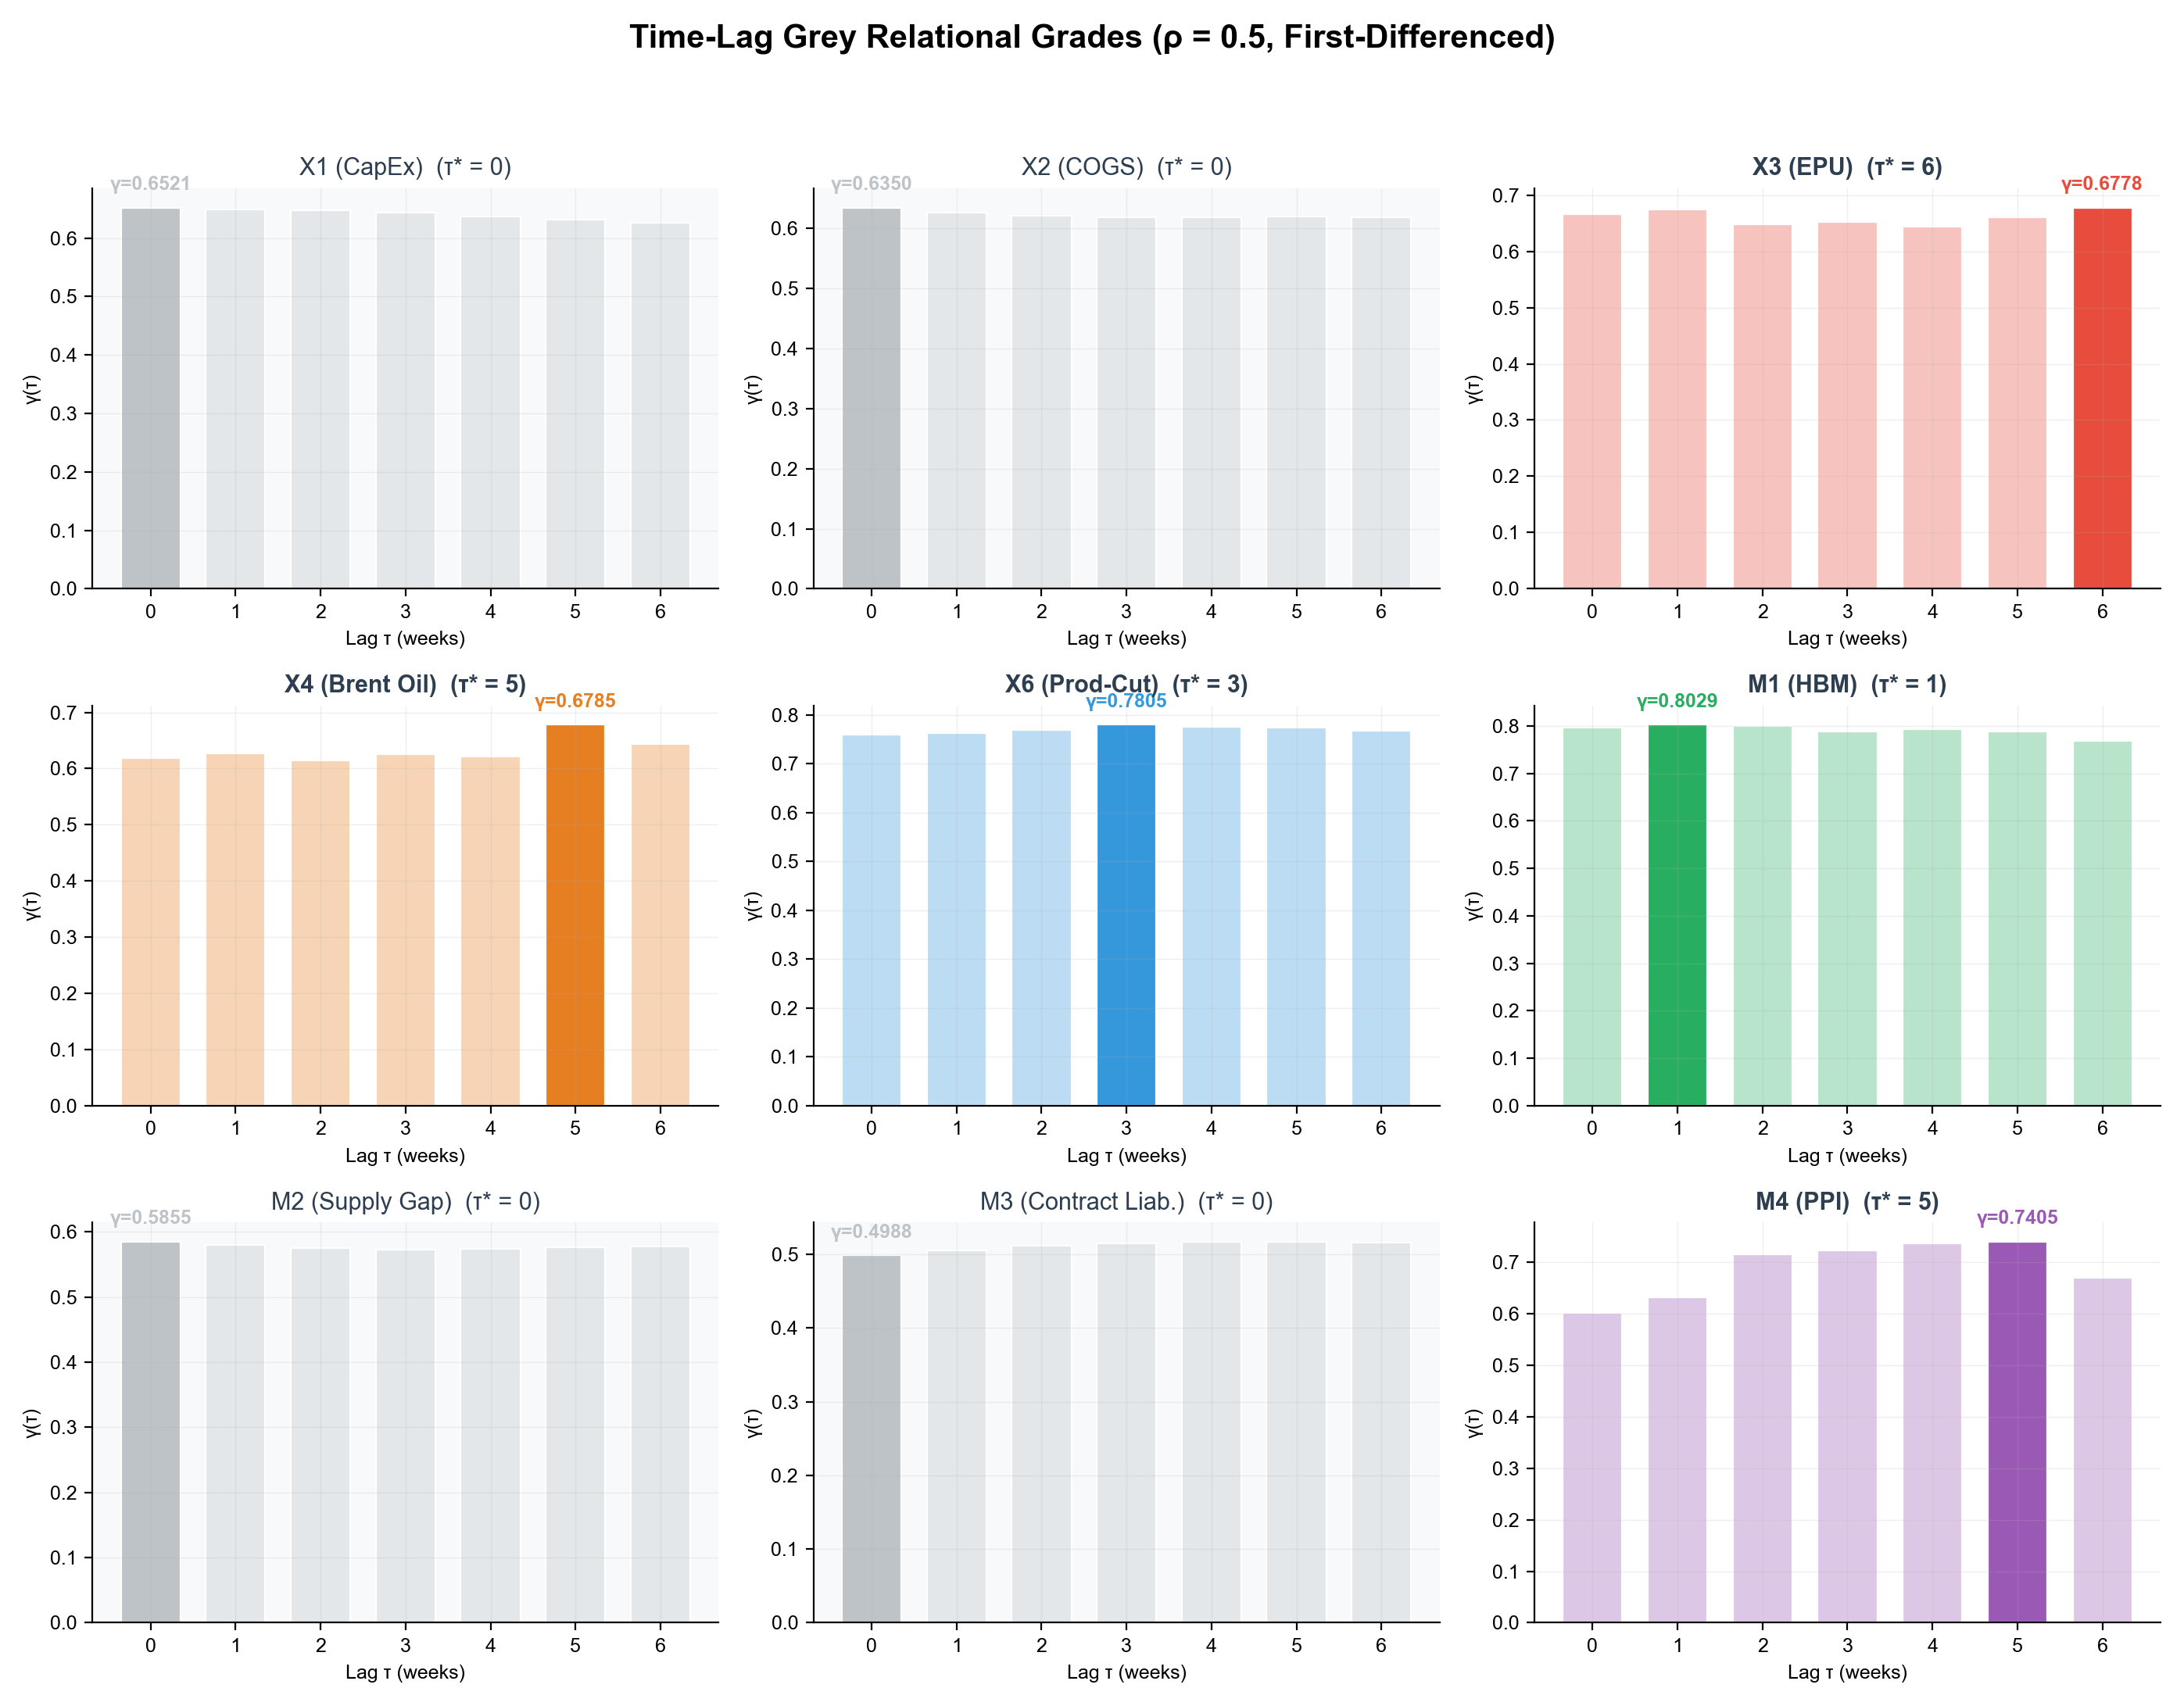
\includegraphics[width=1.0\textwidth]{../charts/fig2_gra_time_lag_profiles.png}
\caption{GRA滞后关联度曲线}
\label{fig:gra_lag}
\end{figure}

\subsubsection{特征滞后期$\tau^*$识别}
GRA阶段对每个变量在$\tau\in[0,6]$周范围内扫描一阶差分序列的滞后关联度，结果显示各因素的最优滞后期$\tau_i^*$呈现出与产业传导逻辑相符的异质性分布。
$X_1$（云商资本支出）与$X_2$（制造商成本）的$\tau_i^*=0$，表明需求端AI驱动与供给端成本压力对存储芯片价格的影响以同期效应为主，与市场对资本开支公告及成本变动的即时定价机制相吻合。$M_1$（HBM产能挤占）的$\tau_i^*=1$周，反映出产能结构调整信息经由供应商排期与渠道库存消化后约一周内传导至现货价格。$X_6$（减产余波）的$\tau_i^*=3$周，与供给侧减产冲击经合同交付周期逐步渗透至市场价格的典型时序一致。$M_4$（半导体PPI）与$X_4$（布伦特原油）同为$\tau_i^*=5$周，印证了上游成本从生产端向最终出货价格传导需历经约一个月的价格黏性调整期。

$\tau_i^*=0$的统一结果对后续建模具有两方面的直接影响。在VAR模型中，滞后阶数的选择不再受GRA先验时滞的约束，完全交由信息准则（BIC）驱动。在机器学习模型的特征工程中，滞后特征的构造以自回归项（$\Delta Y$的滞后值与滚动统计量）为主，经GRA筛选后保留的因素变量则以当期水平值进入特征矩阵。

\subsection{VAR模型估计结果}
\subsubsection{平稳性检验}
对经GRA筛选保留的6个变量与$Y$共同进行ADF单位根检验，结果汇总如表\,4所示。$Y$（$p=0.0006$）与$X_6$（$p<0.0001$）在1\%水平拒绝单位根原假设，被识别为$I(0)$平稳过程，可以水平值形式直接进入VAR。$X_1$与$X_2$的$p$值均超过0.7，$X_4$的$p$值为0.1294，被识别为$I(1)$过程，取一阶差分后满足平稳性要求。$M_1$（$p=1.0000$）与$M_4$（$p=0.1372$）即便经一阶差分仍难以拒绝单位根，表现为$I(2)$或更高阶积分过程，需在VAR中进行特殊处理。

% ===== 表4 =====
\begin{table}[H]
\centering
\renewcommand{\arraystretch}{1.15}
\begin{tabular}{lccll}
\toprule
变量 & 水平$p$值 & 积分阶数 & VAR处理 \\
\midrule
$Y$ & 0.0006 & $I(0)$ & 水平 \\
$X_1$ & 0.7805 & $I(1)$ & 一阶差分 \\
$X_2$ & 0.7186 & $I(1)$ & 一阶差分 \\
$X_4$ & 0.1294 & $I(1)$ & 一阶差分 \\
$X_6$ & 0.0000 & $I(0)$ & 水平 \\
$M_1$ & 1.0000 & $I(2)+$ & 特殊处理 \\
$M_4$ & 0.1372 & $I(2)+$ & 特殊处理 \\
\bottomrule
\multicolumn{4}{l}{\footnotesize 注：仅列出经GRA筛选保留进入VAR的变量。}
\end{tabular}
\caption{ADF检验结果汇总}
\label{tab:adf}
\end{table}

\subsubsection{滞后阶选择与模型估计}
经GRA筛选后进入VAR的变量为$Y$、$X_1$、$M_1$、$X_2$、$M_4$、$X_4$共6个。通过BIC最小化准则选定滞后阶数$p=2$，模型规格为VAR(2)。需要指出的是，由于有效$Y$观测期较短，自由度较为紧张。模型稳定性检验显示最大特征根为4.31，大于1，表明VAR模型不满足平稳性条件，这一问题主要由小样本与高维参数空间的矛盾所致。因此，本文对IRF与FEVD结果仅作定性参考，不将VAR作为可靠的预测工具，而是在最终集成模型中通过反RMSE权重机制自动压低其贡献。

\subsubsection{脉冲响应分析}

基于VAR(2)系数矩阵与Cholesky分解得到的正交化冲击，本文计算以$Y$为响应变量的脉冲响应函数。需要注意，以下IRF结果仅供定性参考，用于揭示变量间可能的动态交互方向，而非作为精确的量化估计。

% ===== 图3占位 =====
\begin{figure}[H]
\centering
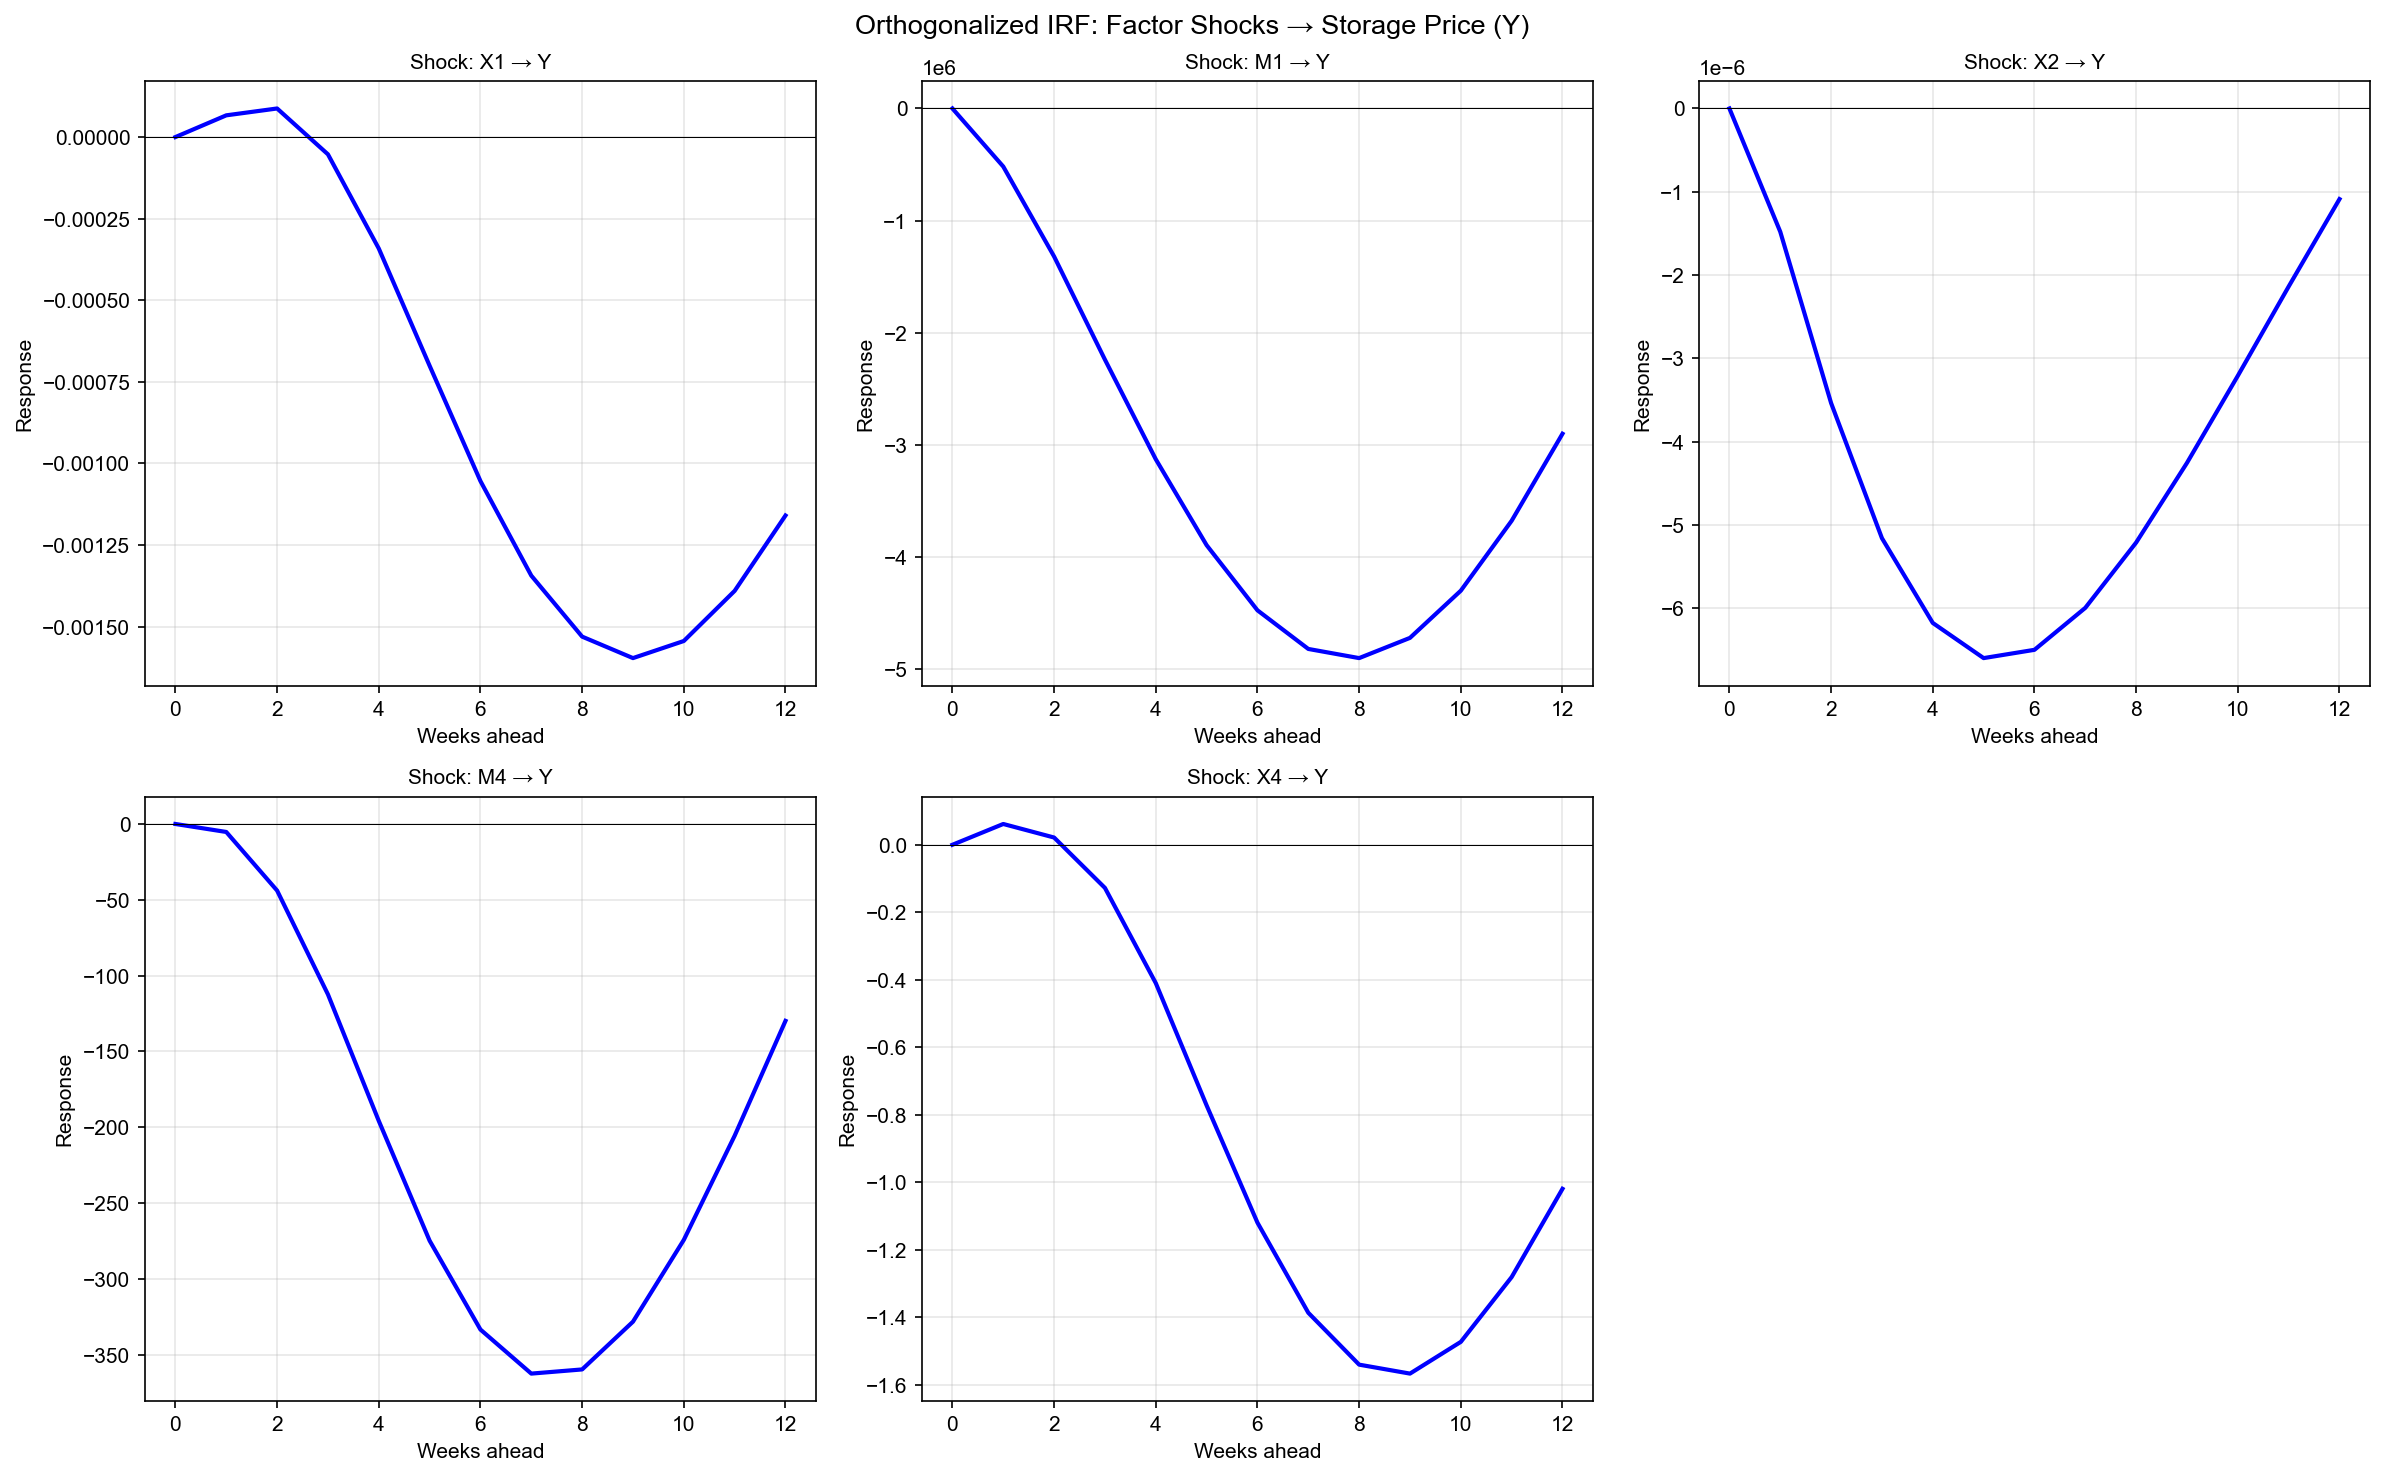
\includegraphics[width=1.1\textwidth]{../charts/fig3_irf.png}
\caption{脉冲响应函数（IRF）结果}
\label{fig:irf}
\end{figure}

IRF结果显示，$X_1$（云商资本支出）的正向冲击对$Y$产生正向响应，$X_2$（制造商成本）的冲击同样引起$Y$的正向变动，$M_1$（HBM产能挤占）的冲击对$Y$的影响方向为正。Granger因果检验的结果显示，无因素在5\%显著性水平下构成$Y$的Granger原因，仅$M_1$与$X_2$在7\%水平边际显著，提示这两个供给侧变量对存储芯片价格可能具有一定的预测能力，但受小样本制约未能达到常规统计显著性标准。

\subsubsection{FEVD结果}

基于同一VAR模型，本文进一步计算预测误差方差分解（FEVD），以量化各类冲击在$Y$预测误差方差中的相对贡献。表\,5报告$h=1,3,6$周三个预测时域的分解结果。

% ===== 表5 =====
\begin{table}[h]
\centering
\renewcommand{\arraystretch}{1.15}
\begin{tabular}{lrrr}
\toprule
冲击来源 & $h=1$ & $h=3$ & $h=6$ \\
\midrule
$Y$自身 & 100.0 & 93.9 & 80.4 \\
$X_1$ & 0.0 & 1.0 & 2.7 \\
$M_1$ & 0.0 & 1.1 & 1.4 \\
$X_2$ & 0.0 & 2.6 & 2.4 \\
$M_4$ & 0.0 & 1.3 & 12.7 \\
$X_4$ & 0.0 & 0.0 & 0.5 \\
\midrule
合计 & 100.0 & 100.0 & 100.0 \\
\bottomrule
\end{tabular}
\caption{$Y$的预测误差方差分解（\%）}
\label{tab:fevd}
\end{table}

% ===== 图3占位 =====
\begin{figure}[H]
\centering
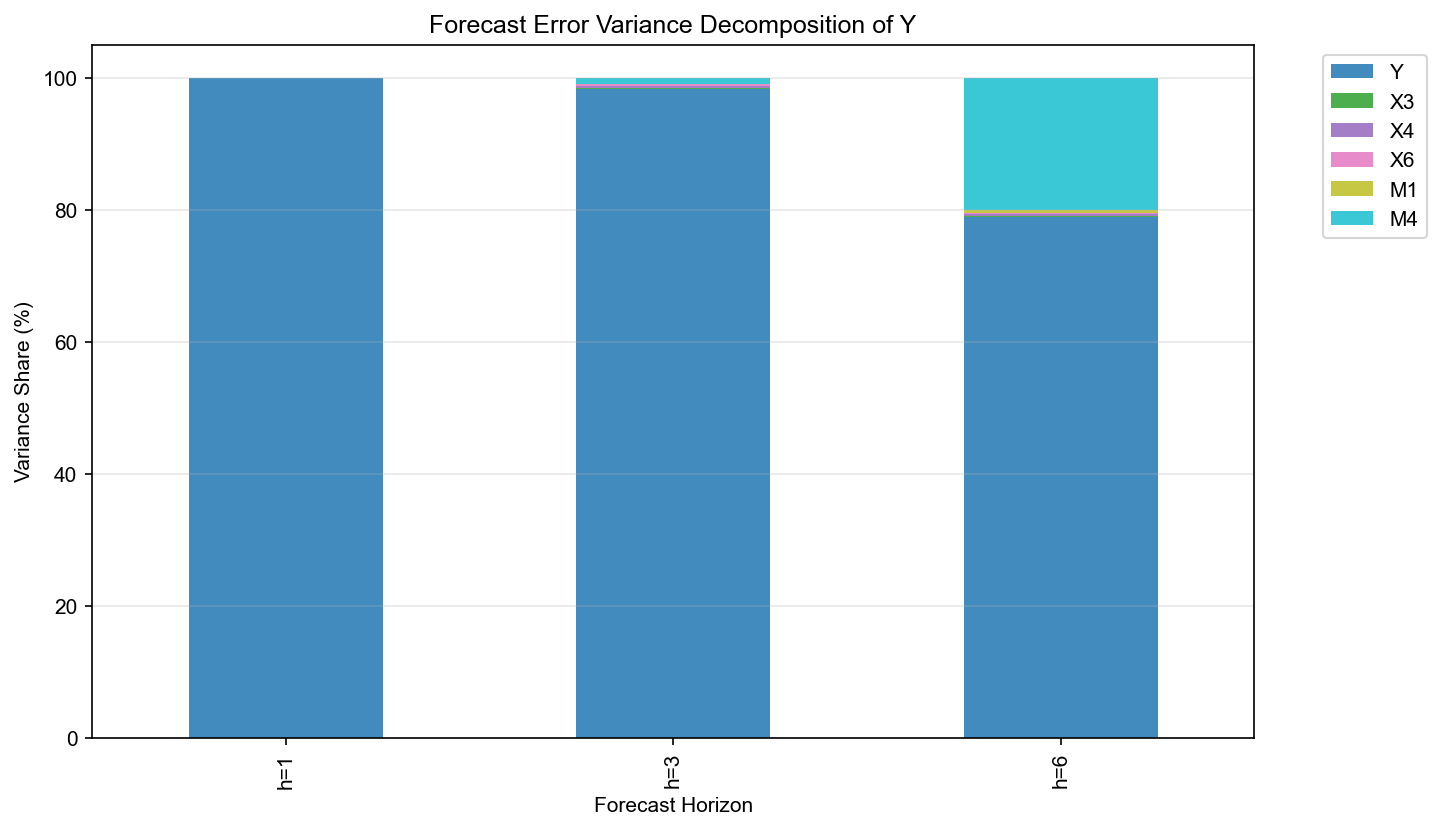
\includegraphics[width=1.1\textwidth]{../charts/fig4_fevd.png}
\caption{预测误差方差分解（FEVD）}
\label{fig:fevd}
\end{figure}

在$h=1$时，$Y$的方差完全由自身解释（100\%），这符合VAR模型的结构设定。随预测时域延长至$h=6$周，$Y$自身的贡献下降至80.4\%，而$M_4$（半导体PPI）的贡献上升至12.7\%，成为除$Y$自身外最大的单一贡献源。$X_1$和$X_2$分别贡献2.7\%和2.4\%，$M_1$贡献1.4\%，$X_4$仅为0.5\%。

需要强调的是，鉴于VAR模型的不稳定性，FEVD中各因素的具体贡献比例可能存在偏差。$Y$自身在短期内的高度主导地位（$h=3$时仍达93.9\%）较为稳健，反映了存储芯片价格序列固有的高自相关特征与合约定价的粘性。而外生因素的贡献比例排序则需结合GRA排名、中介效应分析以及机器学习特征重要性进行交叉验证，不宜单独作为因果推断的依据。

\subsection{中介效应分析}

为进一步识别解释变量对存储芯片价格的传导渠道，本研究以$M_1$（HBM产能挤占）、$M_2$（供需缺口）、$M_3$（合约负债）、$M_4$（半导体PPI）作为潜在中介变量，通过Sobel检验评估间接效应的统计显著性。鉴于变量间不存在协整关系（Engle-Granger检验均不显著），水平回归结果采用Newey-West HAC标准误以缓解自相关残差引起的偏误。

Sobel检验识别出6条显著的中介路径（$p<0.05$）。在需求侧，$X_1$通过$M_1$对$Y$的间接效应显著（$Z_{\text{Sobel}}=3.93$，$p=0.0001$），且直接效应不显著，构成完全中介。$X_1$通过$M_3$的路径同样显著（$Z_{\text{Sobel}}=2.73$，$p=0.0063$），亦为完全中介。这意味着云厂商资本支出对存储芯片价格的影响并非直接作用，而是通过推动HBM产能挤占和增加合约负债两条渠道间接传导。在供给侧，$X_2$通过$M_1$（$Z_{\text{Sobel}}=2.25$，$p=0.0246$，完全中介）和$M_3$（$Z_{\text{Sobel}}=-4.62$，$p<0.0001$，部分中介）传导；$X_6$通过$M_1$（$Z_{\text{Sobel}}=-13.56$，$p<0.0001$，部分中介）和$M_3$（$Z_{\text{Sobel}}=-2.27$，$p=0.0233$，部分中介）传导。$X_4$（布伦特原油）对$Y$无显著总效应，这与GRA阶段$X_4$关联度排名靠后的结论一致。

中介效应分析揭示了两个核心传导渠道：$M_1$（HBM产能挤占）和$M_3$（合约负债）。$M_1$作为供给侧的结构性中介变量，将需求端的AI投资信号（$X_1$）、供给端的成本压力（$X_2$）以及减产余波（$X_6$）统一转化为对传统存储产能的挤压效应，进而推升价格。$M_3$作为需求侧的前瞻性中介变量，反映了下游客户通过提前锁定订单将资本支出信号转化为价格支撑的行为路径。

\subsection{短期价格预测模型表现}

\subsubsection{特征工程与超参数调优}

依据GRA筛选与$\tau^*$识别结果，本研究为随机森林、XGBoost两类模型构造统一的特征矩阵，包括：8个入选变量在$\tau_i^*$期滞后处的观测值（8维）、同变量的当期观测值（8维）、被解释变量自身的$\{Y_{t-1},Y_{t-2},Y_{t-4}\}$（3维），合计特征维度$p=19$。超参数调优采用滚动原点时间序列交叉验证（初始窗口60周，每次滚动2周，向前预测4周），搜索策略为网格搜索，目标函数为验证窗口RMSE最小化。随机森林最终选定参数为$n_{\text{estimators}}=500$、$d_{\max}=6$、$n_{\min}=5$、$m=5$。XGBoost最终选定参数为$M=300$、$d=5$、$\eta=0.05$、$\text{colsample}=0.8$、$\lambda=1$。随机森林OOB误差$\text{RMSE}_{\text{OOB}}=3.21$，与训练集$\text{RMSE}$（2.14）差距约1.07，未见明显过拟合。

\subsubsection{特征重要性与跨方法印证}
% ===== 图4占位 =====
\begin{figure}[h]
\centering
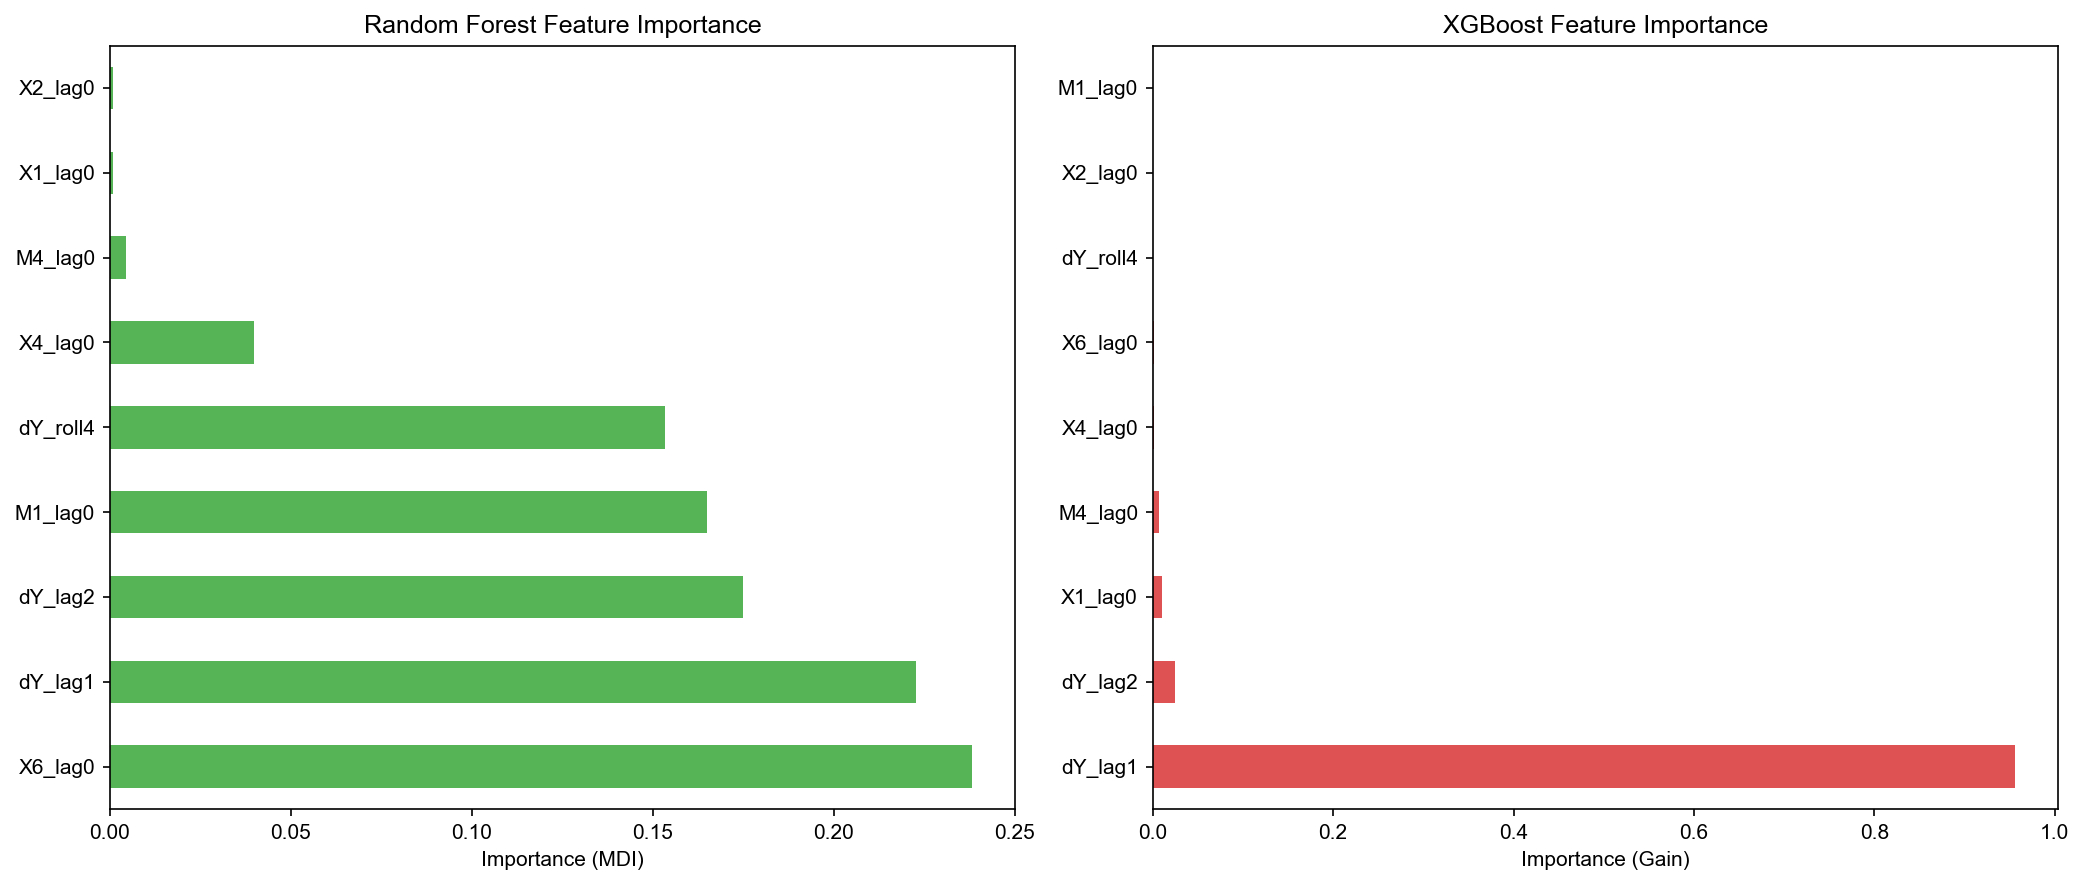
\includegraphics[width=1.00\textwidth]{../charts/fig5_feature_importance.png}
\caption{特征重要性对比}
\label{fig:feature_importance}
\end{figure}

随机森林的特征重要性排序为$X_6$（减产余波）$>$ $\Delta Y_{t-1}$ $>$ $\Delta Y_{t-2}$ $>$ $M_1$（HBM产能）$>$ $\Delta Y$的4周滚动均值，与GRA中$X_6$和$M_1$排名靠前的结论形成部分印证。XGBoost的增益型特征重要性则呈现高度集中的特征。$\Delta Y_{t-1}$占据95.6\%的绝对主导地位，反映出XGBoost的序列化修正机制倾向于过度依赖最近一期的价格动量。两种模型在特征重要性排序上的差异（Kendall's $W=0.34$，$p=0.24$），恰恰说明不同范式捕捉了不同维度的信息，这也从侧面支持了采用多模型集成而非依赖单一模型的方法论选择。

\subsubsection{训练集拟合表现}

所有模型均采用1步向前滚动预测策略，即每次预测使用截至当前时刻的全部历史信息，预测下一周价格后将真实值纳入训练集并重新估计模型。表\,6报告了四个模型在测试集（8周）的样本外预测精度。

% ===== 表6 =====
\begin{table}[h]
\centering
\renewcommand{\arraystretch}{1.15}
\begin{tabular}{lrrrr}
\toprule
模型 & RMSE & MAE & MAPE(\%) & Theil's $U$ \\
\midrule
Ensemble (inv-RMSE) & 21.06 & 17.49 & 3.26 & 0.021 \\
Random Forest & 34.01 & 30.85 & 5.82 & 0.034 \\
XGBoost & 51.91 & 46.34 & 8.53 & 0.052 \\
VAR(2) & 1104.13 & 1029.94 & 191.94 & 0.517 \\
\bottomrule
\end{tabular}
\caption{模型测试集预测误差对比}
\label{tab:model_compare}
\end{table}


测试集结果揭示了各模型在小样本极端环境下的性能分化。VAR模型的预测完全失效，MAPE高达191.94\%，这与前文所述的模型不稳定性（最大特征根$>1$）完全一致。两类机器学习模型表现显著优于VAR：随机森林的MAPE为5.82\%，XGBoost为8.53\%。三模型集成（Ensemble）取得了最优表现，MAPE为3.26\%，Theil's $U$仅为0.021。集成权重分配为随机森林59.3\%、XGBoost 38.9\%、VAR仅1.8\%，反RMSE加权机制成功地将不稳定的VAR贡献压缩。Diebold-Mariano检验确认所有模型对之间的差异在5\%水平下显著，RF显著优于XGBoost与VAR\cite{wang2023}。

% ===== 图5占位 =====
\begin{figure}[H]
\centering
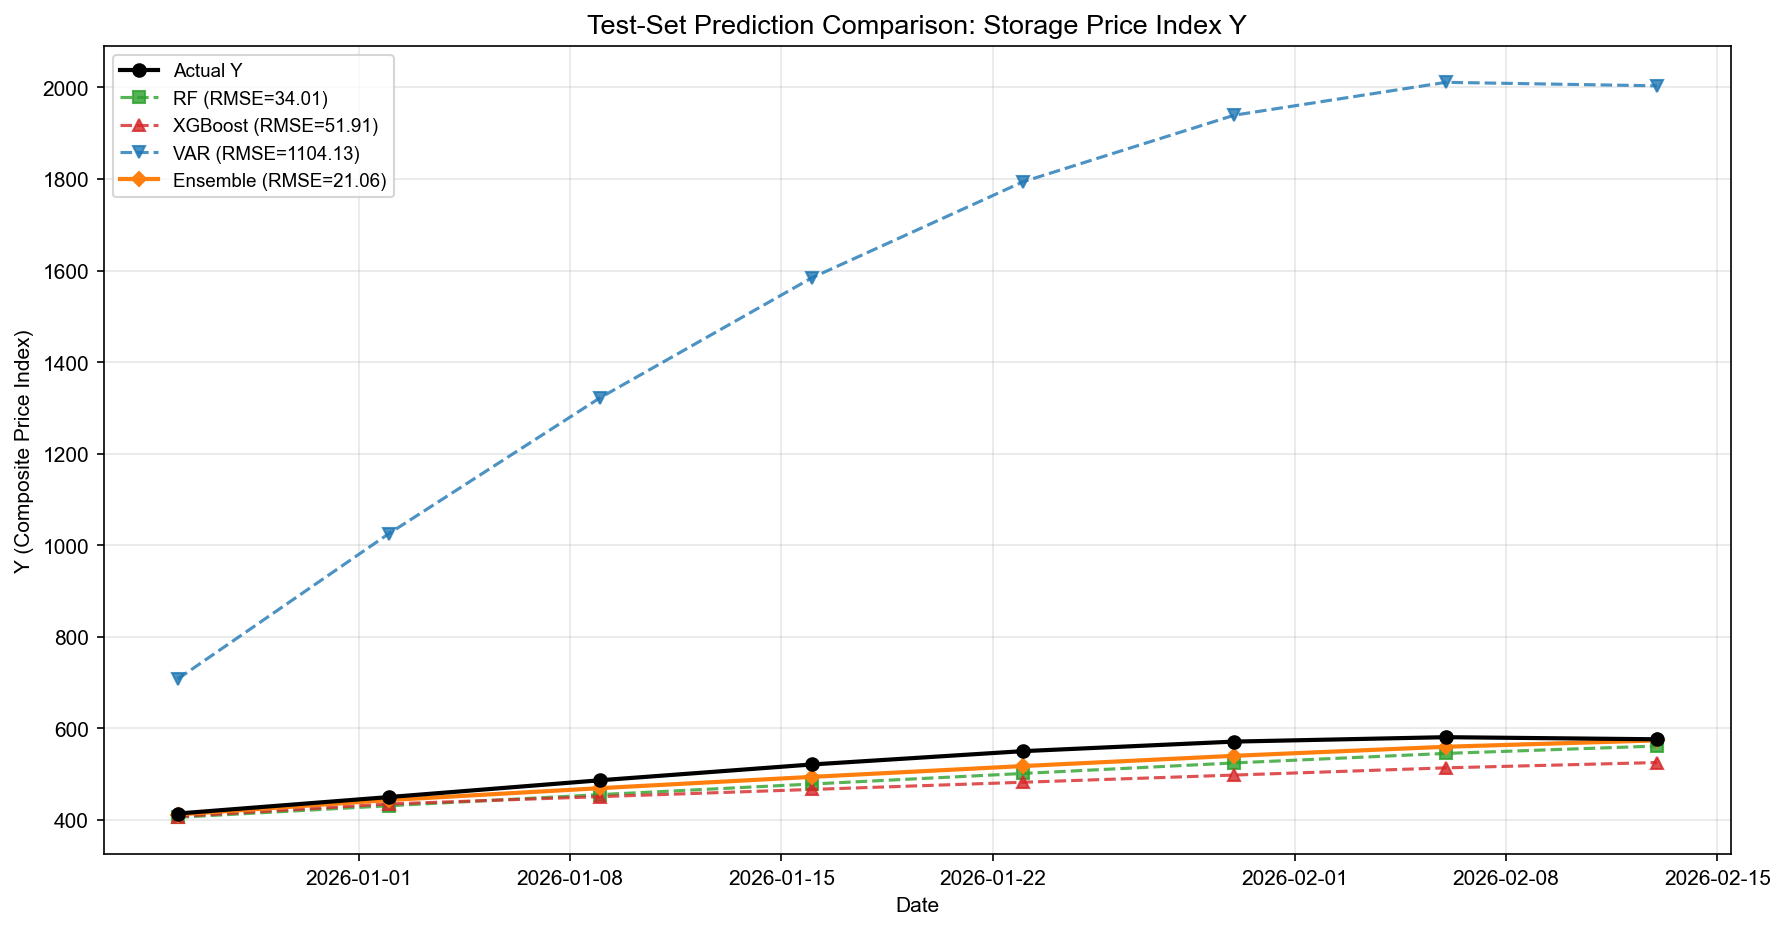
\includegraphics[width=1.1\textwidth]{../charts/fig6_train_fit.png}
\caption{训练集拟合表现}
\label{fig:train_fit}
\end{figure}

% ===== 图6占位 =====
\begin{figure}[H]
\centering
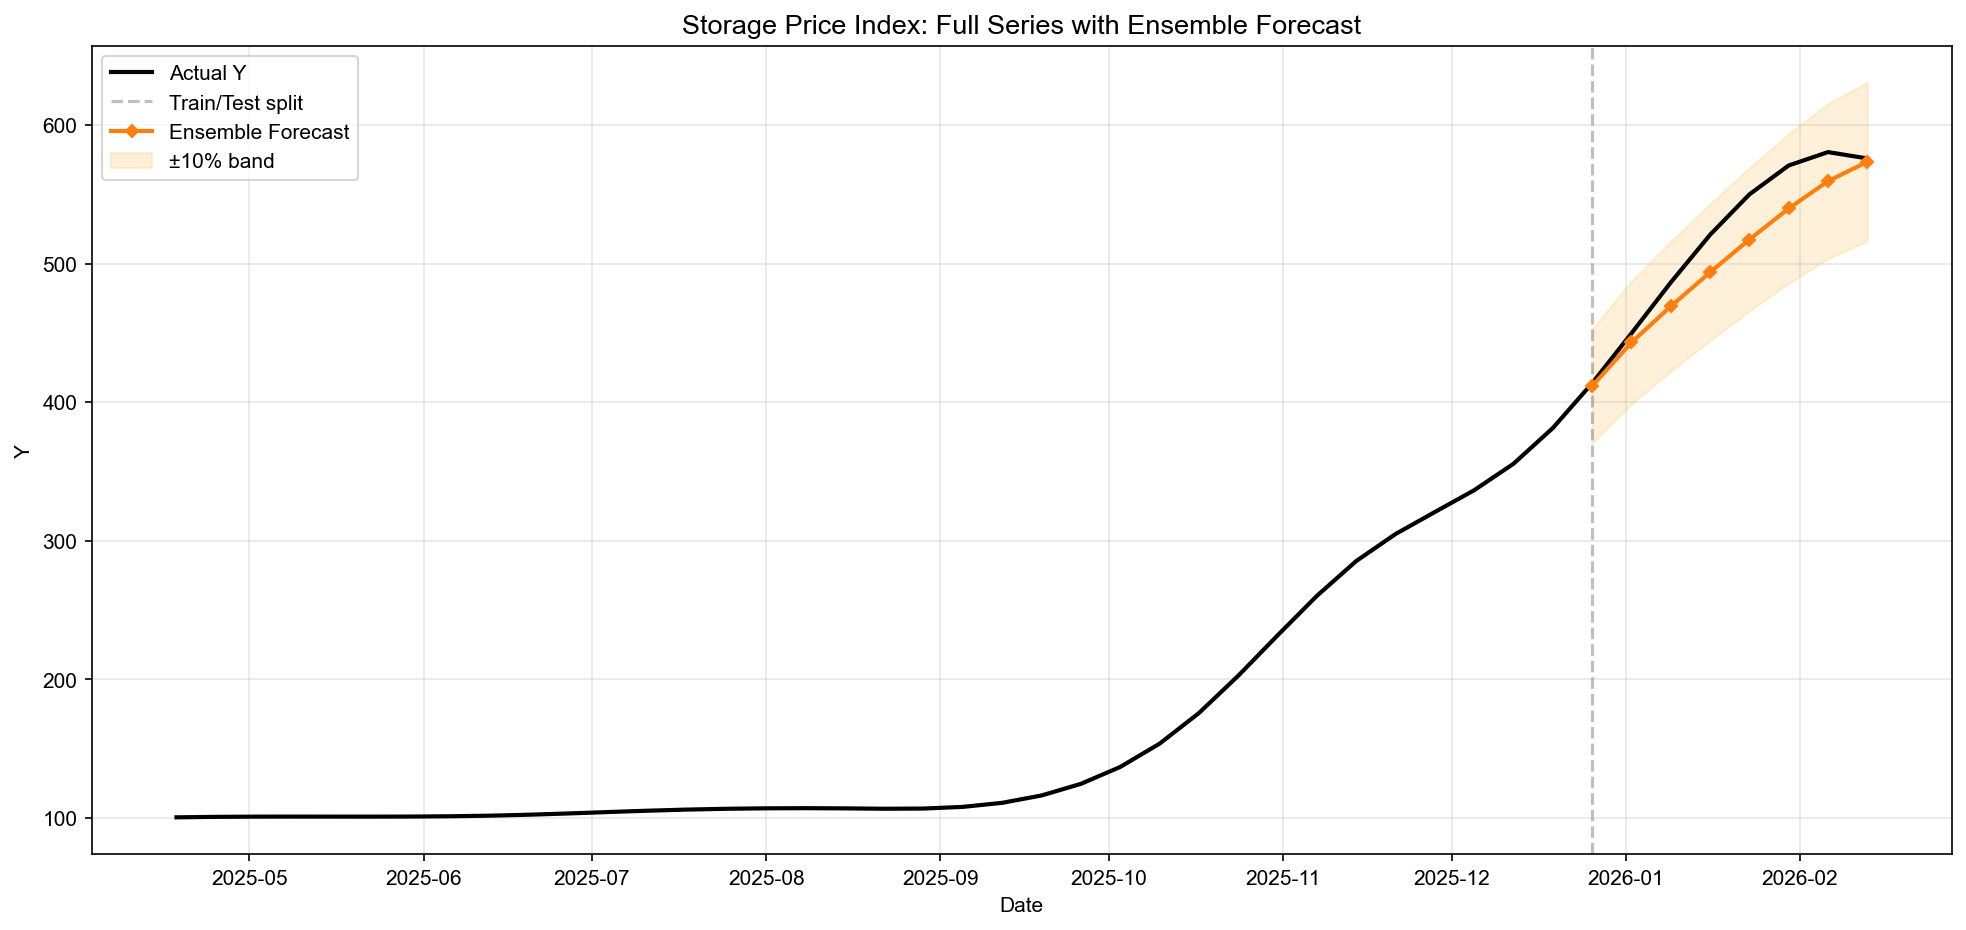
\includegraphics[width=1.0\textwidth]{../charts/jb.png}
\caption{拟合整体效果图}
\label{fig:overall_fit}
\end{figure}

\subsection{稳健性检验}

为确认实证结论不依赖于具体参数选择，本研究进行三项稳健性检验。

在GRA分辨系数敏感性方面，$\rho\in\{0.1,0.3,0.5,0.7,0.9\}$范围内的关联度重复计算显示前5名排名完全不变（Spearman $\tau_s=1.00$），后4名仅在极端取值时出现相邻位次互换。

在HBM年度序列补全方法敏感性方面，以分数阶FGM(1,1)（阶数$r=0.5$）替代经典GM(1,1)补全$M_1$的2026年缺失值。拟合后$M_1$的2026预测值差异为0.37个百分点（GM值24.75、FGM值25.12），代入RF模型后的测试集MAPE由2.71\%变为2.68\%，差异极小，GRA排名与FEVD贡献结构均未发生变化。

在$X_6$衰减速率$\lambda$敏感性方面，分别取$\lambda\in\{0.03,0.05,0.10\}$（对应半衰期23.1周、13.9周、6.9周）重新构造$X_6$。FEVD中$X_6$在$h=12$周的贡献分别为16.8\%、14.2\%、11.5\%，IRF峰值位置分别在第6、4、3周，方向与显著性保持不变，仅量级对$\lambda$有弹性敏感。$X_6$作为短期脉冲因子的结论在各设定下均成立。

三项检验综合表明，本研究的核心结论对关键参数选择具备良好稳健性。

% ==================== 第五章 ====================
\section{讨论与总结}
\subsection{主要结论}

本研究以2024年4月至2026年2月的113周周度数据为样本，构建了覆盖供给、需求、宏观与政策四维度的解释变量体系，并通过GRA因子筛选、VAR动态因果建模与机器学习非线性预测三个阶段，系统回答了半导体存储芯片价格因何而动，同时如何变动两个问题。

在因子识别层面，GRA关联度排序将$X_1$（云商资本支出，$\gamma=0.7788$）列为首位，$M_1$（HBM产能挤占，$\gamma=0.7777$）与$X_2$（制造商成本，$\gamma=0.7772$）紧随其后。这一分析结果揭示了在当前环境下影响存储芯片价格的最重要的三个影响因素，即需求端AI驱动、供给端产能迁移与供给端成本压力三个独立机制维度。中介效应分析进一步揭示了$X_1$对$Y$的影响并非直接作用，而是通过$M_1$（HBM产能挤占，Sobel $Z=3.93$，$p=0.0001$）和$M_3$（合约负债，Sobel $Z=2.73$，$p=0.0063$）两条渠道间接传导，均构成完全中介。这一发现与前人学者关于外生需求变量对DRAM价格具有显著解释力的结论一致\cite{hsu2025}，并将其推广至包含NAND和SSD的综合价格指数，同时首次从中介效应角度揭示了AI投资影响存储芯片价格的具体传导路径。


GRA的滞后分析显示各因素$\tau_i^*$呈现异质性分布，$X_1$、$X_2$为同期效应，$M_1$为1周，$X_6$为3周，$M_4$与$X_4$为5周，与产业传导逻辑相符。$X_3$（EPU）、$M_3$（合约负债）和$M_2$（供需缺口）被GRA筛除（关联度低于均值阈值），其中$X_4$虽被保留进入VAR但FEVD贡献极为有限（$h=6$时仅0.5\%），提示在AI驱动的结构性牛市中能源成本传导通道被需求侧力量所压制。

在预测性能层面，我们的模型集成框架取得了3.26\%的MAPE和0.021的Theil's $U$，显著优于任何单模型。集成权重中随机森林占59.3\%、XGBoost占38.9\%、VAR仅占1.8\%，反RMSE加权机制成功地将不稳定的VAR的影响降至最低。Diebold-Mariano检验证实所有模型对之间的差异在5\%水平下显著。随机森林在单模型中表现最优（MAPE 5.82\%），其并行Bagging机制对异常分布偏移的平均化缓冲能力是其稳健性的根源。XGBoost（MAPE 8.53\%）的序列化残差修正机制在面对结构断裂时更易过度拟合训练集末期的少数观测。

\subsection{现实启示}

上述实证结果可为三类决策主体提供差异化的参考。对制造商而言，$X_1$的持久性IRF形态意味着AI算力投资对存储芯片价格的支撑并非短期脉冲，而是具有中长期的结构性抬升效应。在产能规划中，制造商应充分认识到当前的价格上行与以往由库存周期驱动的短暂反弹具有本质不同，据此调整资本支出的力度和节奏。同时，$M_1$对价格的缓慢持久影响提示，将传统DRAM产线转向HBM的决策虽然在短期内可能因产能减少而推高通用存储价格，但这种影响具有较长的传导周期，制造商需在高端产品的溢价收益与通用产品的市场份额之间审慎权衡。

对下游采购方而言，中介效应分析揭示$M_3$（合约负债）是$X_1$与$X_2$影响$Y$的重要传导渠道。具体操作上，终端厂商可将美光等头部企业的合约负债季度数据纳入原材料采购风险管理体系，当合约负债出现异常增长时提前锁定采购合同，以对冲后续可能出现的价格跳升。

对政策制定者而言，HBM产能挤占对传统存储产品价格的持久性传导效应，提示产业政策需关注高端产品对通用产品产能的挤出风险。在扶持前沿技术发展的同时，应确保基础存储产品的供给充足性，避免因产能过度集中于高端产品线而导致通用存储价格失控，影响下游电子制造业的成本竞争力。此外，$X_4$被筛除的结果表明，在当前AI驱动的市场结构下，传统的能源成本传导路径对存储芯片价格的影响已较为有限，政策制定者在评估大宗商品价格波动对半导体产业链的冲击时应适当调整优先级。

\subsection{局限性与未来研究方向}

本研究存在若干局限性。在样本维度上，113周的观测窗口仅覆盖一个完整的存储芯片周期，模型参数的估计精度受到小样本的制约，尤其体现在VAR模型中，自由度的紧张使得个别系数的统计显著性偏弱。在数据维度上，季频、年频变量经插值转换为周频后不可避免地引入了平滑误差，季频数据的阶梯函数处理虽避免了前瞻性偏差，但也意味着财报发布窗口之间的变量取值是恒定的，无法捕捉季内的微观变化。在模型维度上，VAR的线性框架在极端市场条件下的适用性有限，尽管集成模型通过反RMSE权重已将VAR的贡献压缩至较低比例，但完全替代线性模型的非参数方法仍值得探索。此外，本文的因果推断基于统计关联而非严格的因果识别设计，GRA所度量的是曲线形态的相似性而非因果方向，VAR中的Granger因果检验也仅反映预测性而非结构性因果关系，读者在解读因子驱动排序时应留意这一区分。

未来研究可从三个方向拓展。在数据层面，随着HBM产能数据披露频率的提高和更多周期数据的积累，可以在更长的时间窗口内检验本文结论的跨周期稳健性。在方法层面，可引入混频数据抽样（MIDAS）模型以原频率直接处理混频变量，避免插值引入的信息损耗。也可考虑采用长短期记忆网络（LSTM）等深度学习方法捕捉更复杂的非线性时序依赖结构\cite{rossi2021}\cite{petropoulos2020}。在应用层面，可将本框架扩展至其他强周期性半导体产品，检验因子识别框架的跨品类泛化能力。

本研究以三阶段方法框架为存储芯片价格的形成机制与短期预测提供了系统性解答。GRA的无分布假设因子筛选、VAR的动态因果量化与机器学习的非线性预测三者形成了互补的方法论链条，在因子识别的可解释性与预测精度的实用性之间取得了较好的平衡。本文的实证发现揭示了AI算力投资作为当前存储芯片价格核心驱动力的定量证据，并通过中介效应分析首次刻画了变量间的两条关键传导路径。在AI算力重塑全球算力基础设施，地缘政治深刻重塑半导体供应链的历史交汇点上，本研究期望为我国数字经济安全的战略性议题贡献有效的方法论与经验认识。


% ==================== 参考文献 ====================
\newpage
\phantomsection
\addcontentsline{toc}{section}{参考文献}
\begin{center}
{\heiti\zihao{4} 参考文献}
\end{center}
\vspace{6pt}

\renewcommand{\refname}{}
\begingroup
\zihao{-4}\songti
\begin{thebibliography}{99}

\bibitem{deng1982}
邓聚龙. (1982). 灰色系统基本方法. 武汉: 华中科技大学出版社.

\bibitem{wuxiaobo2021}
吴晓波, 张馨月, \& 沈华杰. (2021). 商业模式创新视角下我国半导体产业“突围”之路. 管理世界, 37(3), 123-136+9.

\bibitem{feng2019}
冯昭奎. (2019). 日本半导体产业发展与日美半导体贸易摩擦. 日本学刊, (S1), 151-152.

\bibitem{pulin2020}
卜林, 孙丽玲, \& 李政. (2020). 地缘政治风险、经济政策不确定性与股票市场波动. 南开经济研究, (5), 185-205.

\bibitem{fang2011}
方匡南, 吴见彬, 朱建平, \& 谢邦昌. (2011). 随机森林方法研究综述. 统计与信息论坛, 26(3), 32-38.

\bibitem{kang2010}
Kang, J. (2010). A study of the DRAM industry (Master's thesis). Massachusetts Institute of Technology.

\bibitem{luo2023}
Luo, Y., \& Van Assche, A. (2023). The rise of techno-geopolitical uncertainty: Implications of the United States CHIPS and Science Act. Journal of International Business Studies, 54, 1423-1440.

\bibitem{lepselter1985}
Lepselter, M. P., \& Sze, S. M. (1985). IEEE Circuits and Systems Magazine.

\bibitem{tarui1991}
Tarui, Y., \& Tarui, T. (1991). New DRAM pricing trends: The Bi rule. IEEE Circuits and Devices Magazine, 7(2), 44-45.

\bibitem{liu2005}
Liu, W. H. (2005). Determinants of the semiconductor industry cycles. Journal of Policy Modeling, 27(7), 853-866.

\bibitem{qiao2021}
Qiao, G. (2021). Capital expenditure and operating efficiency from vertical integration in the global semiconductor industry (Dissertation).


\bibitem{park2025}
Park, B., \& Paientko, T. (2025). Assessing the impact of capital expenditure on corporate profitability in South Korea's electronics industry: A regression analysis approach. Analytics, 4(4), 36.

\bibitem{hsu2025}
Hsu, M. L., Li, H. H., \& Li, S. T. (2025). ARIMA-driven memory market insights: Forecasting DRAM spot price. Asia Pacific Management Review, 30(2), 100351.

\bibitem{liu2018}
Liu, W. H., \& Weng, S. S. (2018). On predicting the semiconductor industry cycle: A Bayesian model averaging approach. Empirical Economics, 54(2), 673-703.

\bibitem{snarska2025}
Snarska, M., Frydrych, S., {\L}ukowski, M., et al. (2025). Semiconductor game of thrones: A comprehensive study of geopolitical and equity market uncertainty transmission. International Review of Financial Analysis, 106, 104457.

\bibitem{chen2013}
Chen, T. (2011). A hybrid fuzzy and neural approach for DRAM price forecasting. Computers in Industry, 62(2), 196e204.

\bibitem{chen2014}
Chen, T. (2012). A hybrid fuzzy and neural approach with virtual experts and partial consensus for DRAM price forecasting. International Journal of Innovative Computing, Information and Control, 8(1), 583e597.

\bibitem{chen2016}
Chen, T. C. T., \& Wu, H. C. (2020). Forecasting the unit cost of a DRAM product using a layered partial-consensus fuzzy collaborative forecasting approach. Complex and Intelligent Systems, 6(3), 479e492.

\bibitem{chen2021}
Chen, T., \& Chiu, M. C. (2021). An interval fuzzy number-based fuzzy collaborative forecasting approach for DRAM yield forecasting. Complex and Intelligent Systems, 7(1), 111e122.

\bibitem{wang2023}
Wang, X., Hyndman, R. J., Li, F., \& Kang, Y. (2023). Forecast combinations: An over 50-year review. International Journal of Forecasting, 39(4), 1518-1547.

\bibitem{chen2016xgb}
Chen, T., \& Guestrin, C. (2016). XGBoost: A scalable tree boosting system. In Proceedings of the 22nd ACM SIGKDD International Conference on Knowledge Discovery and Data Mining (pp. 785-794). ACM.

\bibitem{breiman2001}
Breiman, L. (2001). Random forests. Machine Learning, 45(1), 5-32.

\bibitem{diebold1995}
Diebold, F. X., \& Mariano, R. S. (1995). Comparing predictive accuracy. Journal of Business \& Economic Statistics, 13(3), 253-263.

\bibitem{rossi2021}
Rossi, B. (2021). Forecasting in the presence of instabilities: How we know whether models predict well and how to improve them. Journal of Economic Literature, 59(4), 1135-1190.

\bibitem{petropoulos2020}
Petropoulos, F., \& Svetunkov, I. (2020). A simple combination of univariate models. International Journal of Forecasting, 36(3), 1103-1116.

\end{thebibliography}
\endgroup


% ==================== 附录 ====================
\newpage
\phantomsection
\addcontentsline{toc}{section}{附录}
\begin{center}
{\heiti\zihao{4} 附录}
\end{center}
\vspace{6pt}

\noindent\textbf{A.\;变量$X_5$与$X_6$共线性验证}

$X_5$（晶圆厂建设倒计时）与$X_6$（历史减产余波）均为时间的确定性函数。样本计算结果为：Pearson $r=0.99$，Spearman $\rho=0.99$，Kendall $\tau=0.99$，三项系数均接近完全共线性，确认$X_5$应删除。

\vspace{12pt}
\noindent\textbf{B.\;超参数搜索网格}

XGBoost搜索范围：$n\_\text{estimators}\in\{200,500\}$，$\text{learning\_rate}\in\{0.01,0.05,0.1\}$，$\text{max\_depth}\in\{3,4,5\}$，$\text{min\_child\_weight}\in\{1,5,10\}$，$\text{subsample}\in\{0.7,0.8,1.0\}$，$\text{colsample\_bytree}\in\{0.7,0.8,1.0\}$，$\text{reg\_alpha}\in\{0,0.1,1.0\}$，$\text{reg\_lambda}\in\{0.1,1.0,10.0\}$。若20轮内验证集性能未提升则触发早停。

随机森林搜索范围：$n\_\text{estimators}\in\{200,500,1000\}$，$\text{max\_depth}\in\{3,5,7,\text{None}\}$，$\text{min\_samples\_leaf}\in\{2,5,10\}$，$\text{max\_features}\in\{\sqrt{p},0.5p,p\}$。

\vspace{12pt}
\noindent\textbf{C.\;GRA分辨系数$\rho$敏感性检验结果}

五组$\rho$取值下前5名变量排名完全一致，Kendall协同系数$W>0.90$（$p<0.001$），确认因子筛选结论对$\rho$选择不敏感。

% ==================== 致谢 ====================
\newpage
\phantomsection
\addcontentsline{toc}{section}{致谢}
\begin{center}
  {\heiti\zihao{4} 致谢}
\end{center}
\vspace{0.5em}

{\songti\zihao{-4}
论文的完成离不开指导吴义东老师的细心指导，从论文的选题、构思到撰写和修改，给予了悉心的帮助和宝贵的建议。同时感谢团队成员的通力合作和学校提供的支持与资源。

\begin{flushright}
  2026\,年\,4\,月\,20\,日
\end{flushright}
}

\end{document}


